\documentclass[12pt,a4paper,notitlepage]{article}
\usepackage[utf8]{inputenc}
\usepackage[english]{babel}
\usepackage[T1]{fontenc}
\usepackage[backend=biber,
			style=authoryear-comp,
			isbn=false,
			doi=false,
			bibstyle=authoryear,
			natbib,
			]{biblatex}
\usepackage{eurosym}
\usepackage{enumitem}
\usepackage{url}
\usepackage{blindtext}
\usepackage{hyperref}
\usepackage{breakurl}
\usepackage{amsmath}
\usepackage{titling}
\usepackage{amsfonts}
\usepackage{amssymb}
\usepackage{pgfplots}
\usepackage{caption}
\usepackage{subcaption}
\usepackage{graphicx}
\usepackage{dcolumn}
\usepackage{tikz-3dplot}
\usepackage{subcaption}
\usepackage{float}
\usepackage{adjustbox}
\usepackage{multirow,rotating}
\usepackage[autostyle]{csquotes}
\usepackage[toc,page]{appendix}
\usepackage{lscape}
\usepackage{todonotes}
\usepackage{booktabs}
\usepackage{multirow}
\usepackage{bm}
\usepackage{eurosym}
\usepackage{pdflscape}

\addbibresource{Textmining.bib}

\begin{document}

\section{Introduction}

Pluralism is an essential principle of democratic societies. An important pillar of this principle is an opinion-forming process that incorporates as many different perspectives as possible. For the process of forming opinions, information conveyed by the media, in particular the mass media of journalism, plays a decisive role. They create the preconditions for making the social and cultural diversity of modern societies visible and manageable. Securing the diversity of opinion-forming processes and preventing concentration processes in the media sector is an essential prerequisite for a functioning democracy. 

Media outlets (TV, Radio, Newspaper) usually operate in two-sided markets, where they serve two customer groups (content consumer and advertiser) that are connected via indirect network effects. The new developments in digital media provide new opportunities and challenges for media outlets. The costs of providing and disseminating information have been reduced and the speed of information exchange has increased enormously. At first glance, these developments seem to have a positive effect on the provision of information. However, it also means that the incentive for media to produce primary information declines since the Internet has reduced the marginal utility of content. A study of French news websites from 2013 shows that only 38 percent of the online articles contained original content, with the remainder being copies of those originals \citep{cage_information_2017}. At the same time, the number of people who find out about current news on the Internet is increasing. According to a study on the media coverage of the German-speaking population, nearly 40\% of respondents used the internet at least once a week in 2017 to inform themselves about the current news compared to 34\% in 2016 \citep{vuma_arbeitsgemeinschaft_verbrauchs-_und_medienanalyse_verbrauchs-_2017}. Recognizing the importance of media pluralism, the European Commission has endorsed several initiatives to discuss and promote media diversity in the European Union \citep{_media_2014}. 

This paper examines the media pluralism in the market for German-language online news. More specifically, I use a data set of German online news articles about domestic politics dated from 01.06.2017 to 01.03.2018 from seven German news content providers. German federal elections took place on 24th of September 2017 and the formation of the government has taken up a period of about five month. The articles considered here thus inform their readers both about the election promises of the parties (before the election) and about the coalition talks (after the election). They thus make an important contribution to the public's opinion-forming process. The empirical strategy follows a novel approach combining "the two Ts": Topic and Tone \citep{hansen_shocking_2016}. That is, first the topics covered in the articles are identified, to find out how these topics are discussed (tone). The final step is to check whether the tonality of reporting is reflected in the survey results on voting preferences. More precisely, the research strategy is as follows:

\begin{enumerate}
	\item\label{item_1} \textbf{Discovering Topics (Section \ref{subsection_topic})} To discover the latent topics in the corpus, the structural topic modeling (STM) developed by \citet{roberts_model_2016} is applied. The STM is an unsupervised machine learning approach that models topics as multinomial distributions of words and documents as multinomial distributions of topics, allowing to incorporate external variables that effect both, topical content and topical prevalence. I estimate a model, where the newswire service is included as a control for both the topical content and the topical prevalence. The result of the generative process of STM are the posterior distributions for topic prevalence and topical content, which can then be used to measure the similarity between the news providers in the further course of the paper: (1) $\beta$ is a $K$-by-$V$ matrix (where $K=$ number of topics and $V=$ vocabulary) containing the probability distribution for topic $k$ over the words in the predefined vocabulary. (2) $\theta$ is a $D$-by-$V$ matrix of the document-topic distributions, where the entry $\theta_{dk}$ can be interpreted as the proportion of words in document $d$ which arise from topic $k$, or rather as the probability that document $d$ deals about topic $k$. As the prevalence of topics are allowed to vary across news wires, the posterior topic-probability $\theta_{dk}$ of an article (document) can be used to estimate the conditional expectation of topic prevalence for given article characteristics. 
	\item\label{item_2} \textbf{Measuring Tone (Section \ref{subsection_tone}) After assigning a topic to each article (document), a dictionary-based sentiment analysis is conducted to estimate how topics are discussed differently by different news wires.
	\item\label{item_3} \textbf{Comparing with polls} In order to check whether the transmitted content from the online media is reflected in the voting preferences, we compare the values from \ref{item_2} with the survey values of the Sunday survey ("Sonntagsumfrage") graphically and mathematically. The latter is done by means of correlations. Therefore, no causal relationships are calculated.
	
\end{enumerate}

Approach \ref{item_1} has been used in \citet{roberts_model_2016}, among others, to examine differences in the content of news providers. However, I extend the analysis by comparing the sentiment score for a given topic between the news provider, to identify which topics are discussed similar or differently (\ref{item_2}). \citet{hansen_shocking_2016} applied a similar approach to a dataset of 142 FOMC decision statements to measure the effect of those statements on macroeconomic variables. An additional extension is the comparison with current poll values (\ref{item_3}). 

The remaining course of the paper is as follows: In Section \ref{ch_onlinenews} the characteristics of the market for online news in Germany are outlined. The data used to conduct the model is described in Section \ref{ch_data}. Section \ref{ch_model} explains the generative process of the structural topic model as well as the selected parameters to run the model. The empirical analysis containing the above mentioned steps is conducted in Section \ref{ch_empirical}. 
 
% ----------------------
% the online news market
% ----------------------
\section{The online news market}\label{ch_onlinenews}

The market for media content in Germany is characterized by the coexistence of public and private broadcasters. By shifting media content to the Internet, the dual system, which has been shaping the German television and radio landscape since the introduction of private broadcasting in the early 1980s, is facing a radical change. Since 2000, public broadcasting has expanded its range of services, particularly in the digital media sector. In 2017, 22 own websites and 100 apps were operated by public broadcasters on which they offer their content. As a result, public broadcasting no longer only competes with private television and radio stations, but also enters the market for online news. In the following, the characteristics of the market for online news in Germany are briefly described. 

Private media outlets naturally appear as two-sided platforms, that allow interaction between two categories of consumers: audiences and advertisers. As the demand on both consumer-sides are linked via indirect network externalities, the market in which media outlets operate are referred to as two-sided or multi-sided markets. The theoretical literature on two-sided markets originates from the analysis of credit card markets \citep{rochet_platform_2003} and was later transferred to the concept of other industries, such as dating agencies, real estate agents, and internet “business-to-business” websites \citep{caillaud_chicken_2003}. The basic concept of two-sided markets was already discussed decades ago in several economic studies, especially on media markets \citep{corden_maximisation_1952}, \citep{gustafsson_circulation_1978}, \citep{blair_pricing_1993}. However, comprehensive analyses have only been carried out in the last ten years, starting with the works of \citet{rochet_platform_2003}, \citet{evans_empirical_2003} and \citet{armstrong_competition_2006}.

Advertising-supported media such as online newspapers are typical examples of two-sided markets where the newspaper can be conceived as platforms that allow interaction between audiences ("eyeballs") and advertisers. The newspaper creates (or buys) content to attract viewers which in turn attract advertisers who pay for readers' attention \citep{evans_industrial_2005}. The size and characteristics of the audience has a positive effect on the advertisers' willingness to pay, as advertisements are typically sold based on cost per viewer, often expressed in terms of the cost of reaching a thousand viewers (CPM). Advertising can also have an effect on the recipients, which can be either negative or positive, depending on the quality of the advertising. Based on the strength of the indirect network effects, private publishers maximize their revenue by balancing the demand from advertisers and subscribers using different business models \citep{evans_economics_2008}. Many traditional newspapers follow the subscription/advertising model, where the publisher charges both market sides: The audience pays a fee to obtain access to the content, and advertisers pay to obtain access to the viewers. Many online news agencies provide part of their editorial content for free and hide another, more exclusive part behind a paywall. However, since the Internet has considerably simplified the possibilities for obtaining information and thus reduced the marginal utility of content, such a business model can only be efficient if the content behind the paywall is very exclusive. As a result, many publishers rely on a free-media model, in which the publishers do not charge viewers for access to the media at all, in order to attract as many eyeballs as possible to their platform, and thus, exploit the indirect network effects on the advertising site. In fact, most advertising-financed online magazines earn a large part of their gross margin from advertising \citep{evans_industrial_2005}. In order to maximize their profits, these companies have an interest in attracting as many readers as possible. In addition to the quantity of the audience, the demographic characteristics of recipients also have an influence on the willingness to pay on the advertiser site. Online advertising makes it possible to target ads to particular consumers in real time.
 
The two-sided market structure of the private news market results in news platforms striving to choose their content in such a way that its reach is as large as possible in order to maximize profits from advertising revenues. \citet{steiner_program_1952} concluded, that profit-maximizing media owners may choose to offer the same content, i.e. content aligned with the tastes of the majority. \citep{gabszewicz_press_2001} study the problem of diversity of the political content of newspapers. They find that the maximum differentiation only prevails if the readers sufficiently value the political differentiation between the newspapers the advertising market is small enough. On the other hand, advertising may also have a positive impact on the media, as it enables publishers to report independently of political parties. \citet{ellman_what_2009} analyze a theoretical framework of a two-sided market for newspaper, where readers value accuracy and advertisers value advert-receptive readers. They found that advertising increases the intensity of competition for readers and therefore raises accuracy of media coverage. However, in the monopolistic case, newspapers under-report news that sufficiently reduces advertiser profits. 

Given the crucial role of the media in shaping opinion and promoting democracy, pluralism of opinion and accuracy of information is a major concern of public authorities. Public broadcasting in Germany originated in the post-war period and has always had the task of providing the entire population with independent media. This media offer is intended to guarantee diversity of opinion within the media landscape and to be economically and politically independent. The former is given by the fact that the public media are financed by compulsory fees. To take into account the distinct nature of digital media, the Interstate Broadcasting Agreement (Rundfunkstaatsvertrag) also regulates the scope for action of online services offered by public service broadcasting since 2007. Accordingly, public media are not allowed to distribute purchased content and must - depending on the category of content - set a time limit on its accessibility. In addition, there is a strict advertising ban and prohibition of regional reporting. 

However, given today's media landscape, the role of public media provider and its mandate is questioned. The basic justification for a public media offer can be roughly divided into two categories: On the one hand, possible market failure and on the other hand, ensuring diversity. The former involves the pursuit of non-economic (e. g. democratic, social and cultural) objectives, as well as the provision of information that would not be made available by the market due to a lack of willingness to pay. Ensuring the diversity of media content is intended to counteract possible media bias. As stated above, this paper examines content diversity in the market of online news, by comparing the topic prevalence between the news providers. 

% -----
% Data
% -----
\section{Dataset and data preparation}\label{ch_data}

Figure \ref{fig_reach} shows the largest providers of online news in terms of daily pageviews.\footnote{The figure shows the estimated percentage of daily pageviews on the internet that occurred on a specific website.} It is striking that SPIEGEL ONLINE has the greatest reach over the entire course of time followed by Bild.de. Public websites like Deutschlandfunk.de or Tagesschau.de have a rather small share in that market. 

\begin{figure}[H]
	\caption{Percentage of daily pageviews}
	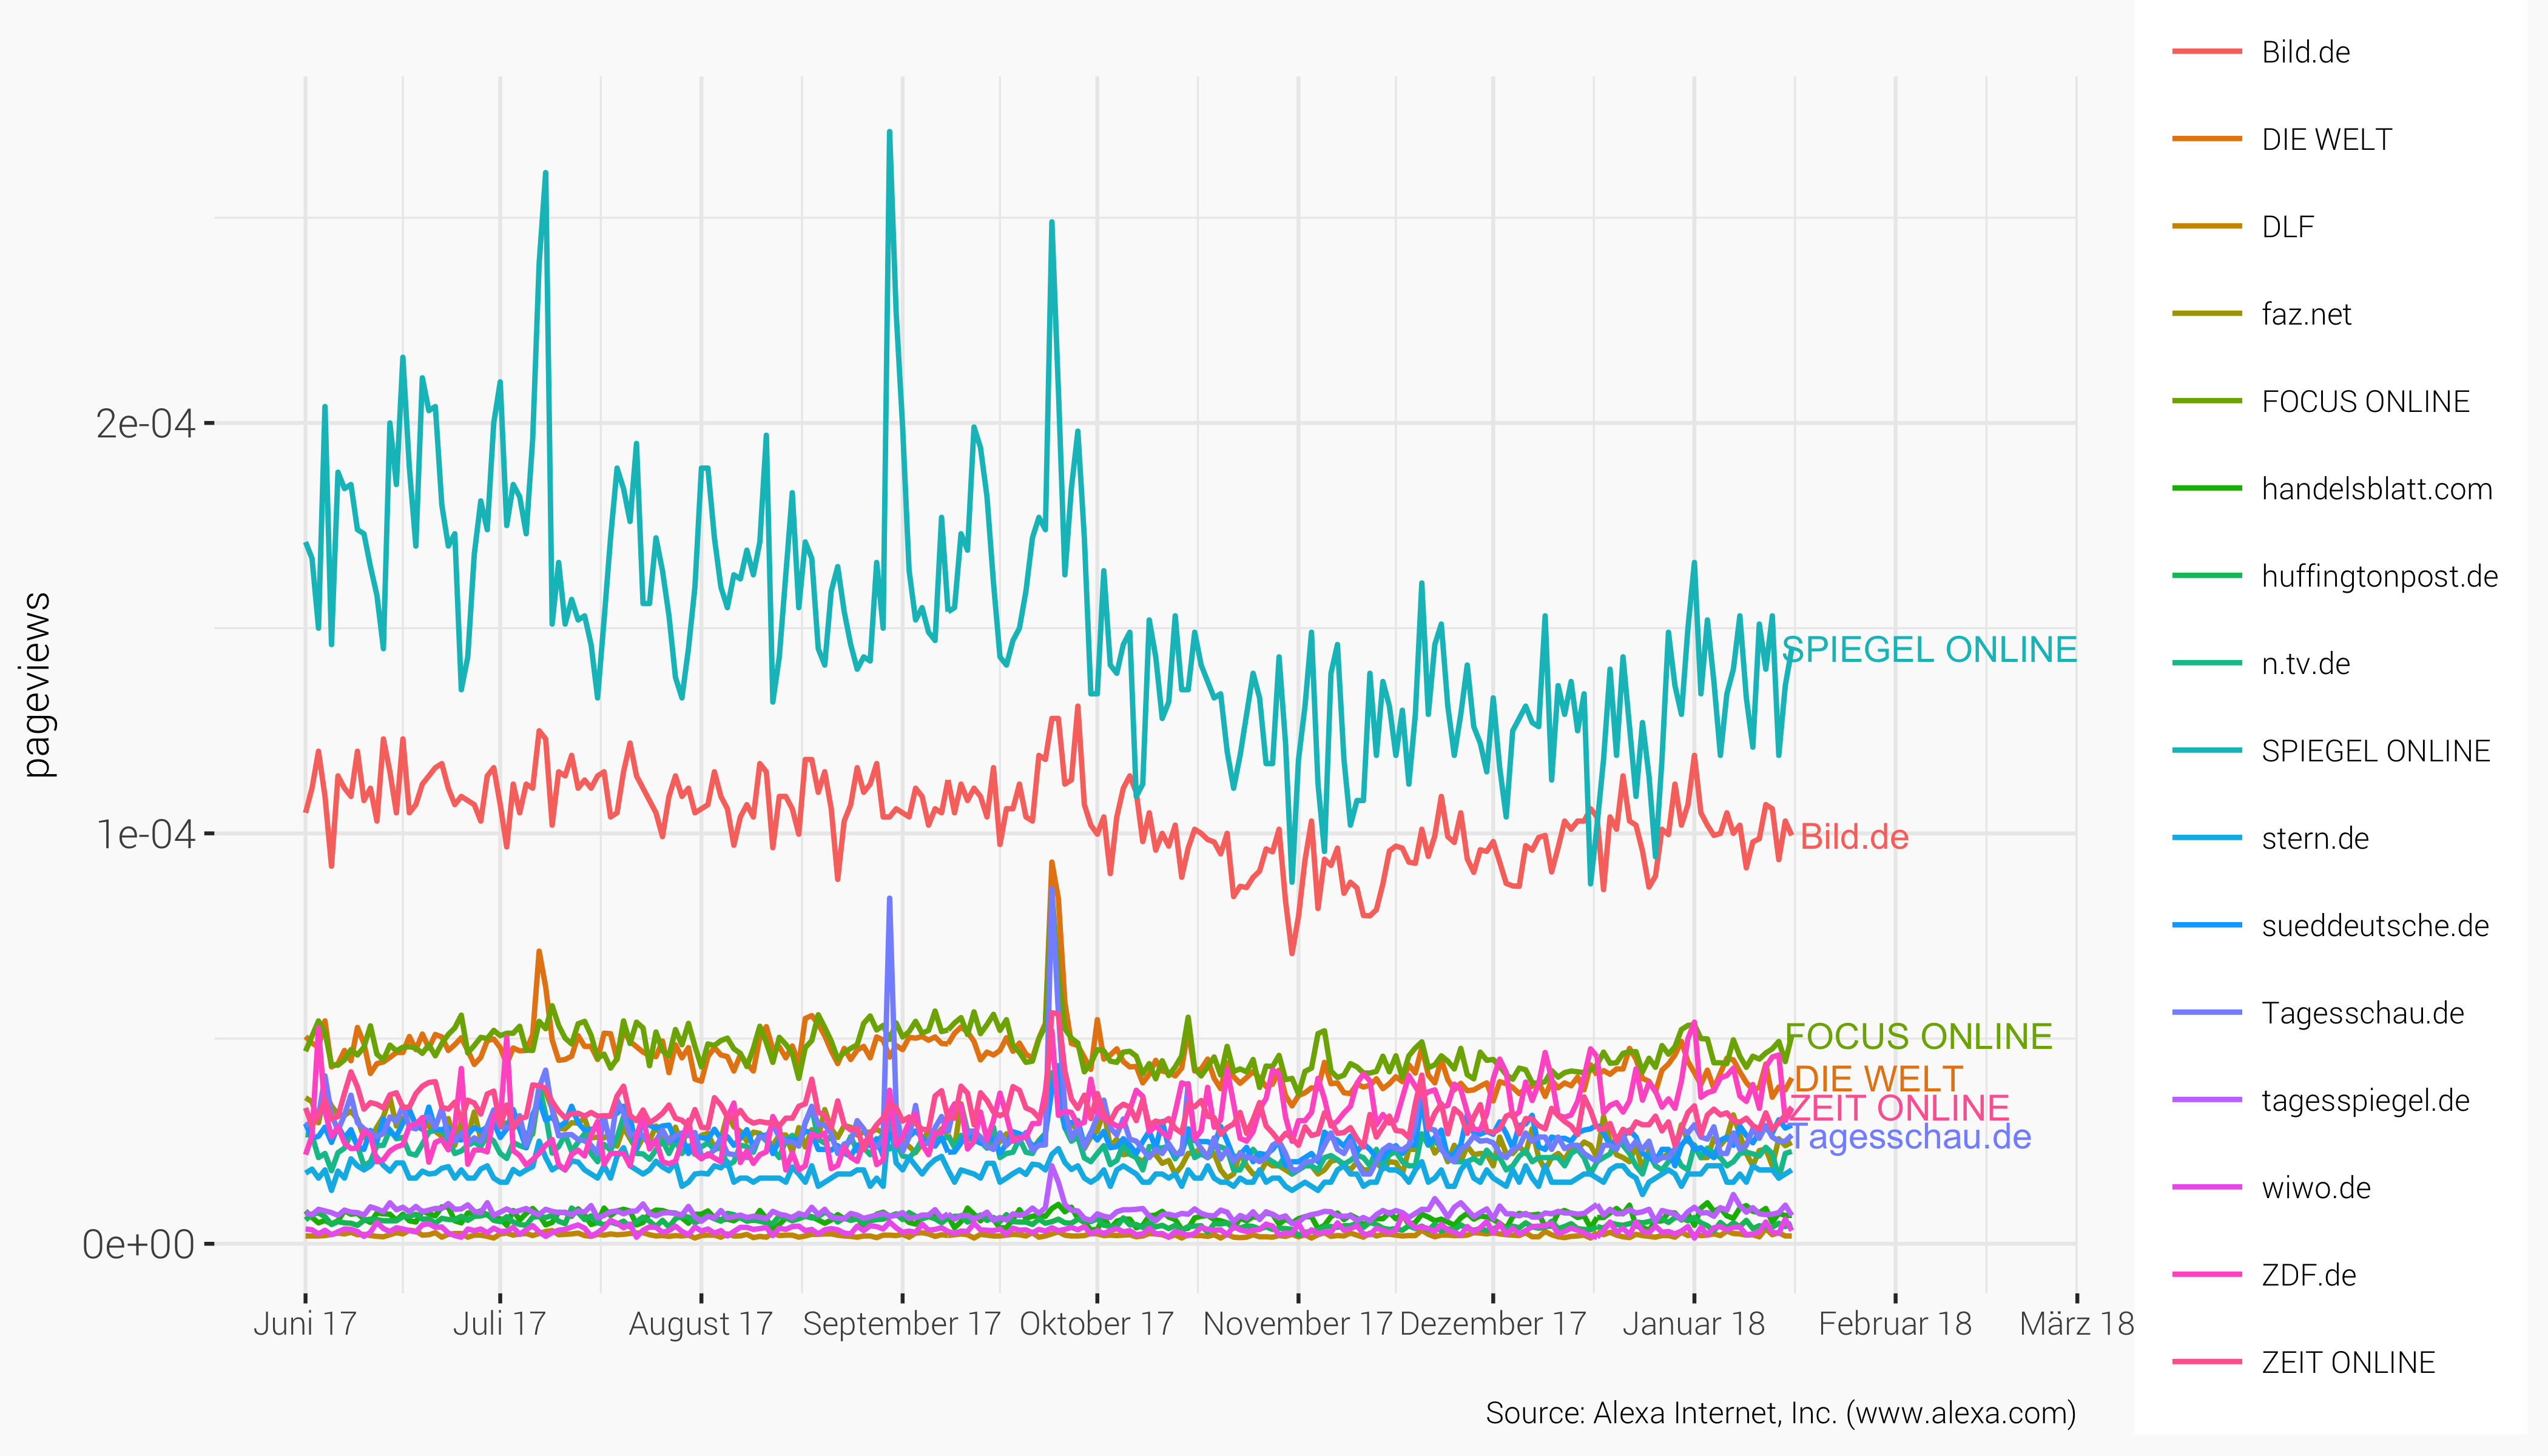
\includegraphics[width=\textwidth]{../figs/reach.png}
	\label{fig_reach}
\end{figure}

I conduct the estimation on a sample of 14,937 online news articles from six news provider about domestic politics\footnote{Bild.de, DIE WELT, FOCUS ONLINE, SPIEGEL ONLINE, Stern.de, ZEIT ONLINE, Tagesschau.de}, of which only Tagesschau.de belongs to the group of public provider. The reason for this is that the content structure of Tagesschau.de is most similar to that of the private providers. ZDF.de offers predominantly video content and DLF website mainly offers audio content in the form of interviews, which makes it hard to include it in the model. The articles are dated from 01.06.2017 to 01.03.2018.\footnote{German federal elections took place on 24th of September 2017.} I first extract all online articles using the the Webhose.io API.\footnote{For more information see https://docs.webhose.io/v1.0/docs/getting-started. The scraping code was written in Python and can be made available on request.} Then all articles from the section "domestic policy" are filtered by checking the URL structure.

Figure \ref{fig_distr1} shows the distribution of the number of articles from the respective news sources by date. There is a high peak around the federal elections on September, 24th.  

\begin{figure}[H]
	\caption{Article distribution...}
	\begin{center}
		\begin{subfigure}[normla]{0.49\textwidth}
			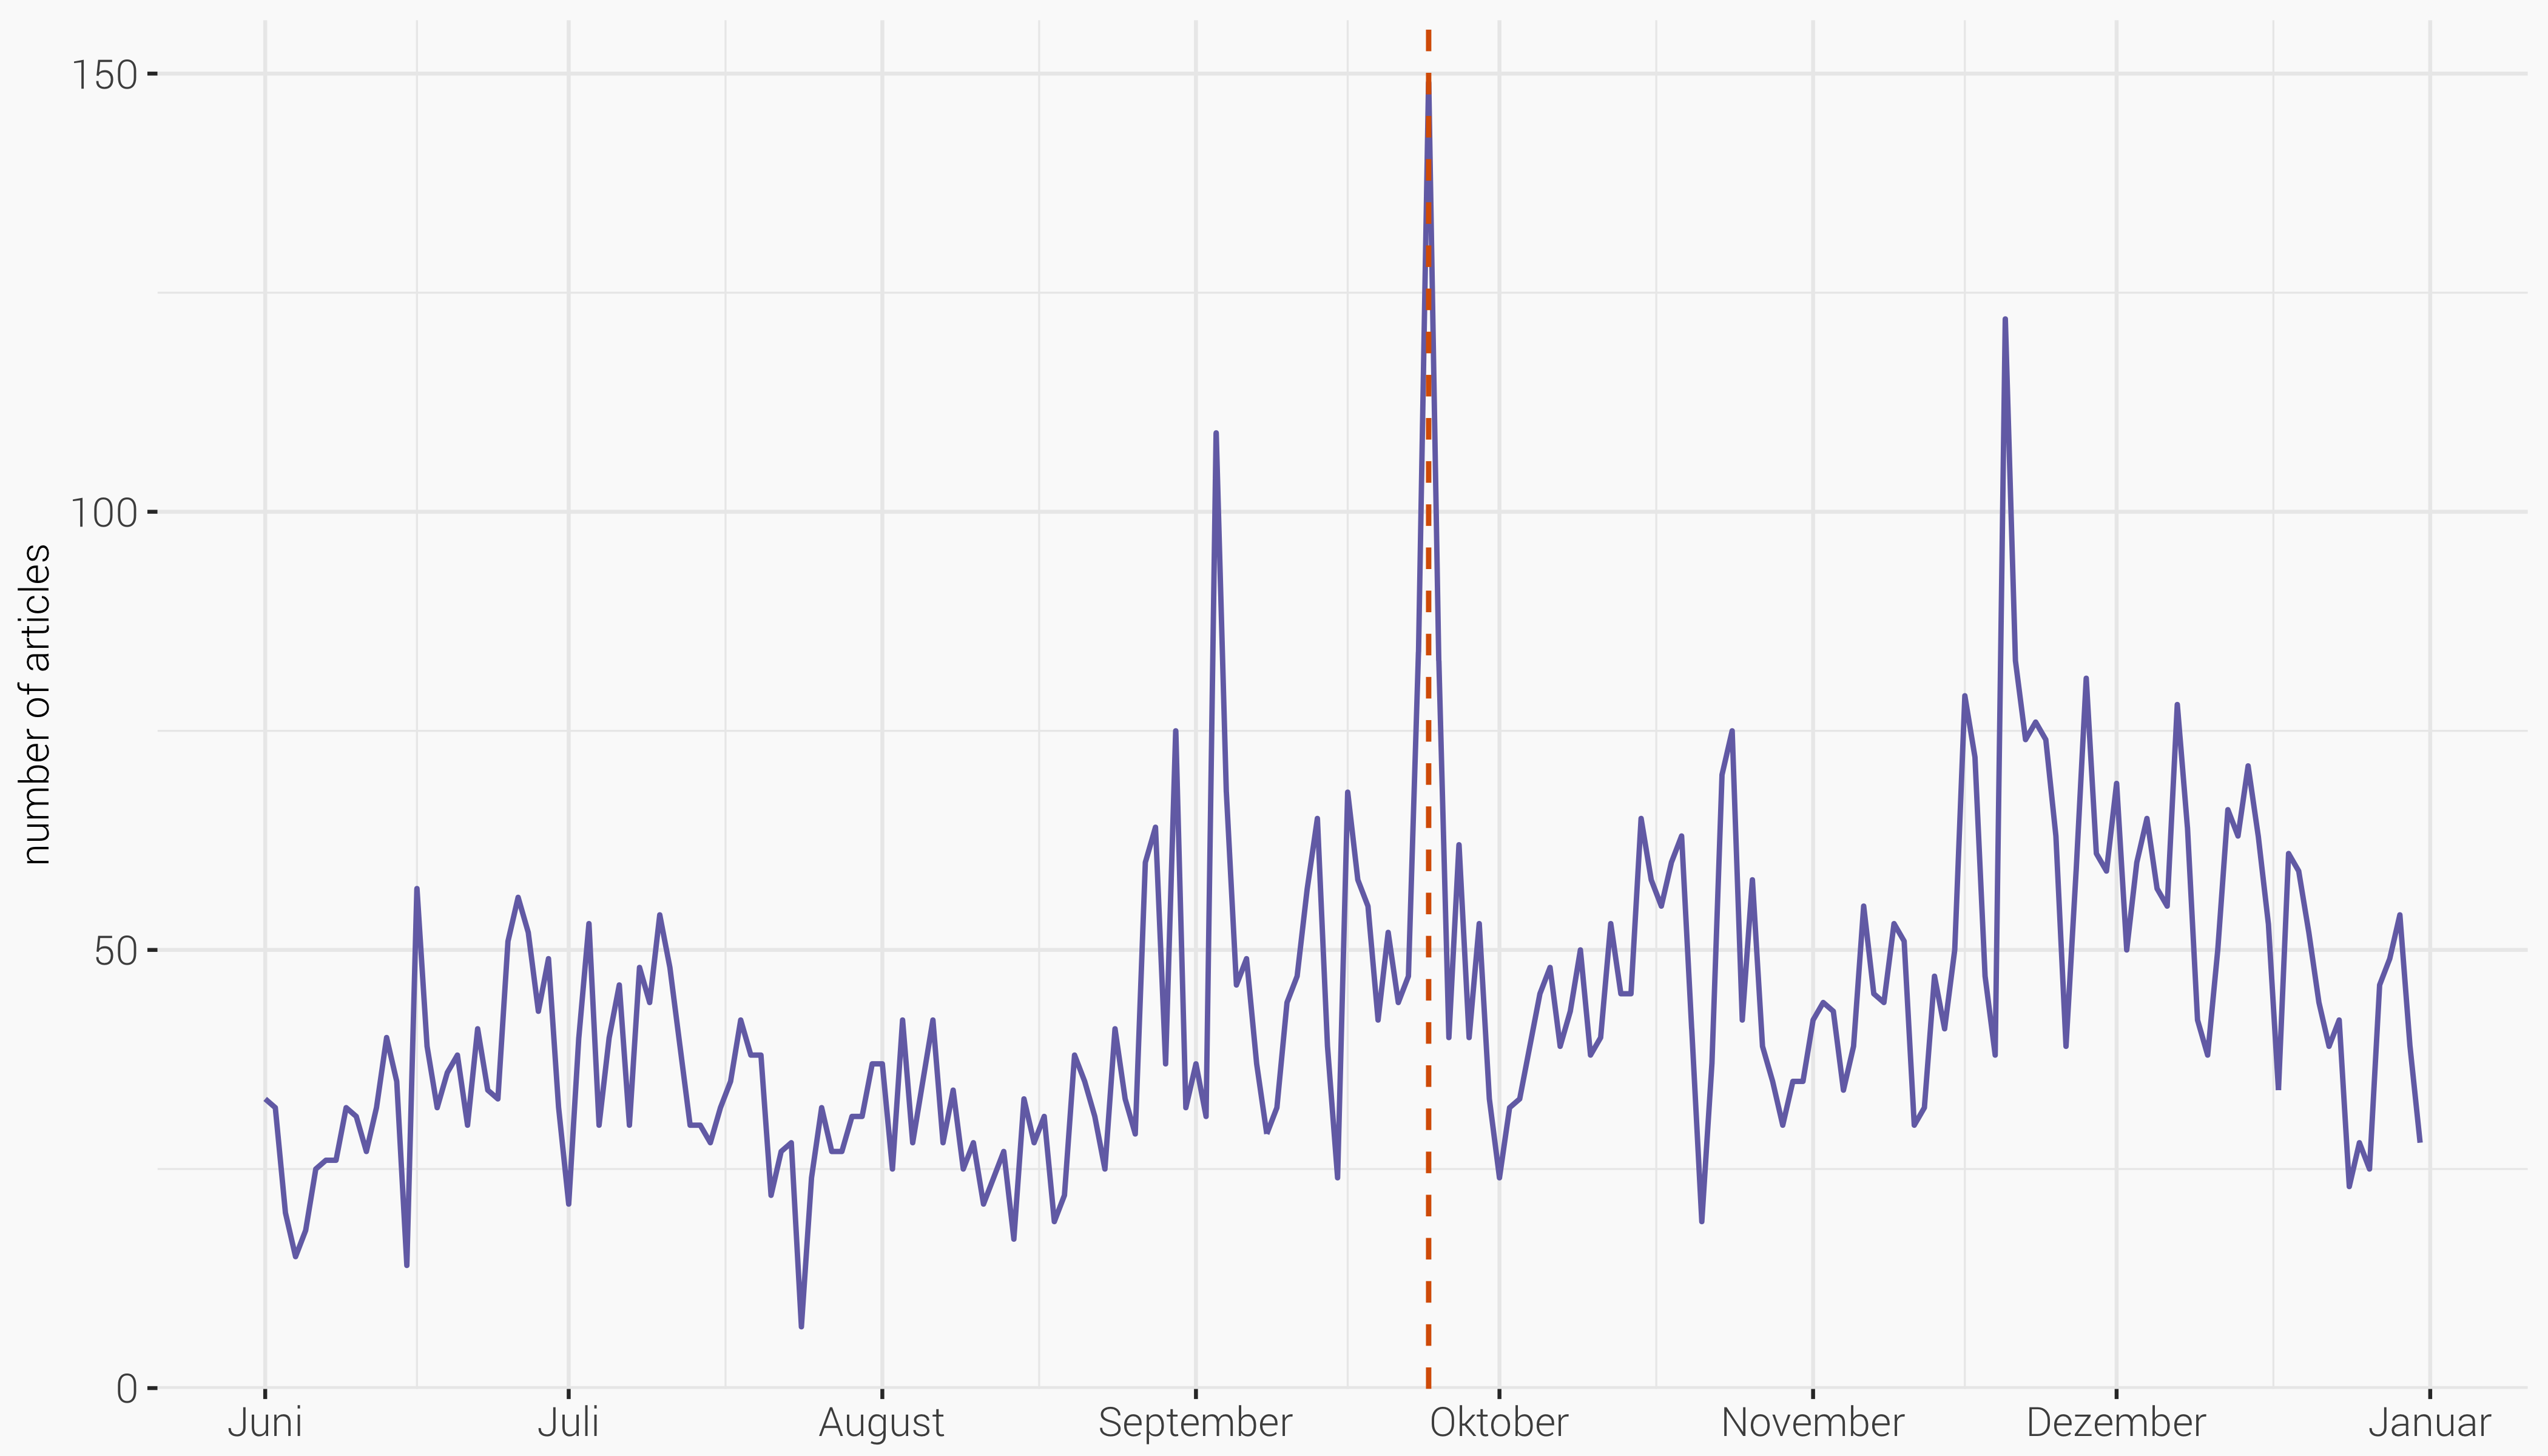
\includegraphics[width=\textwidth]{../figs/timeline.png}
			\caption{...by date}
			\label{fig_distr1}
		\end{subfigure}
		\begin{subfigure}[normla]{0.49\textwidth}
			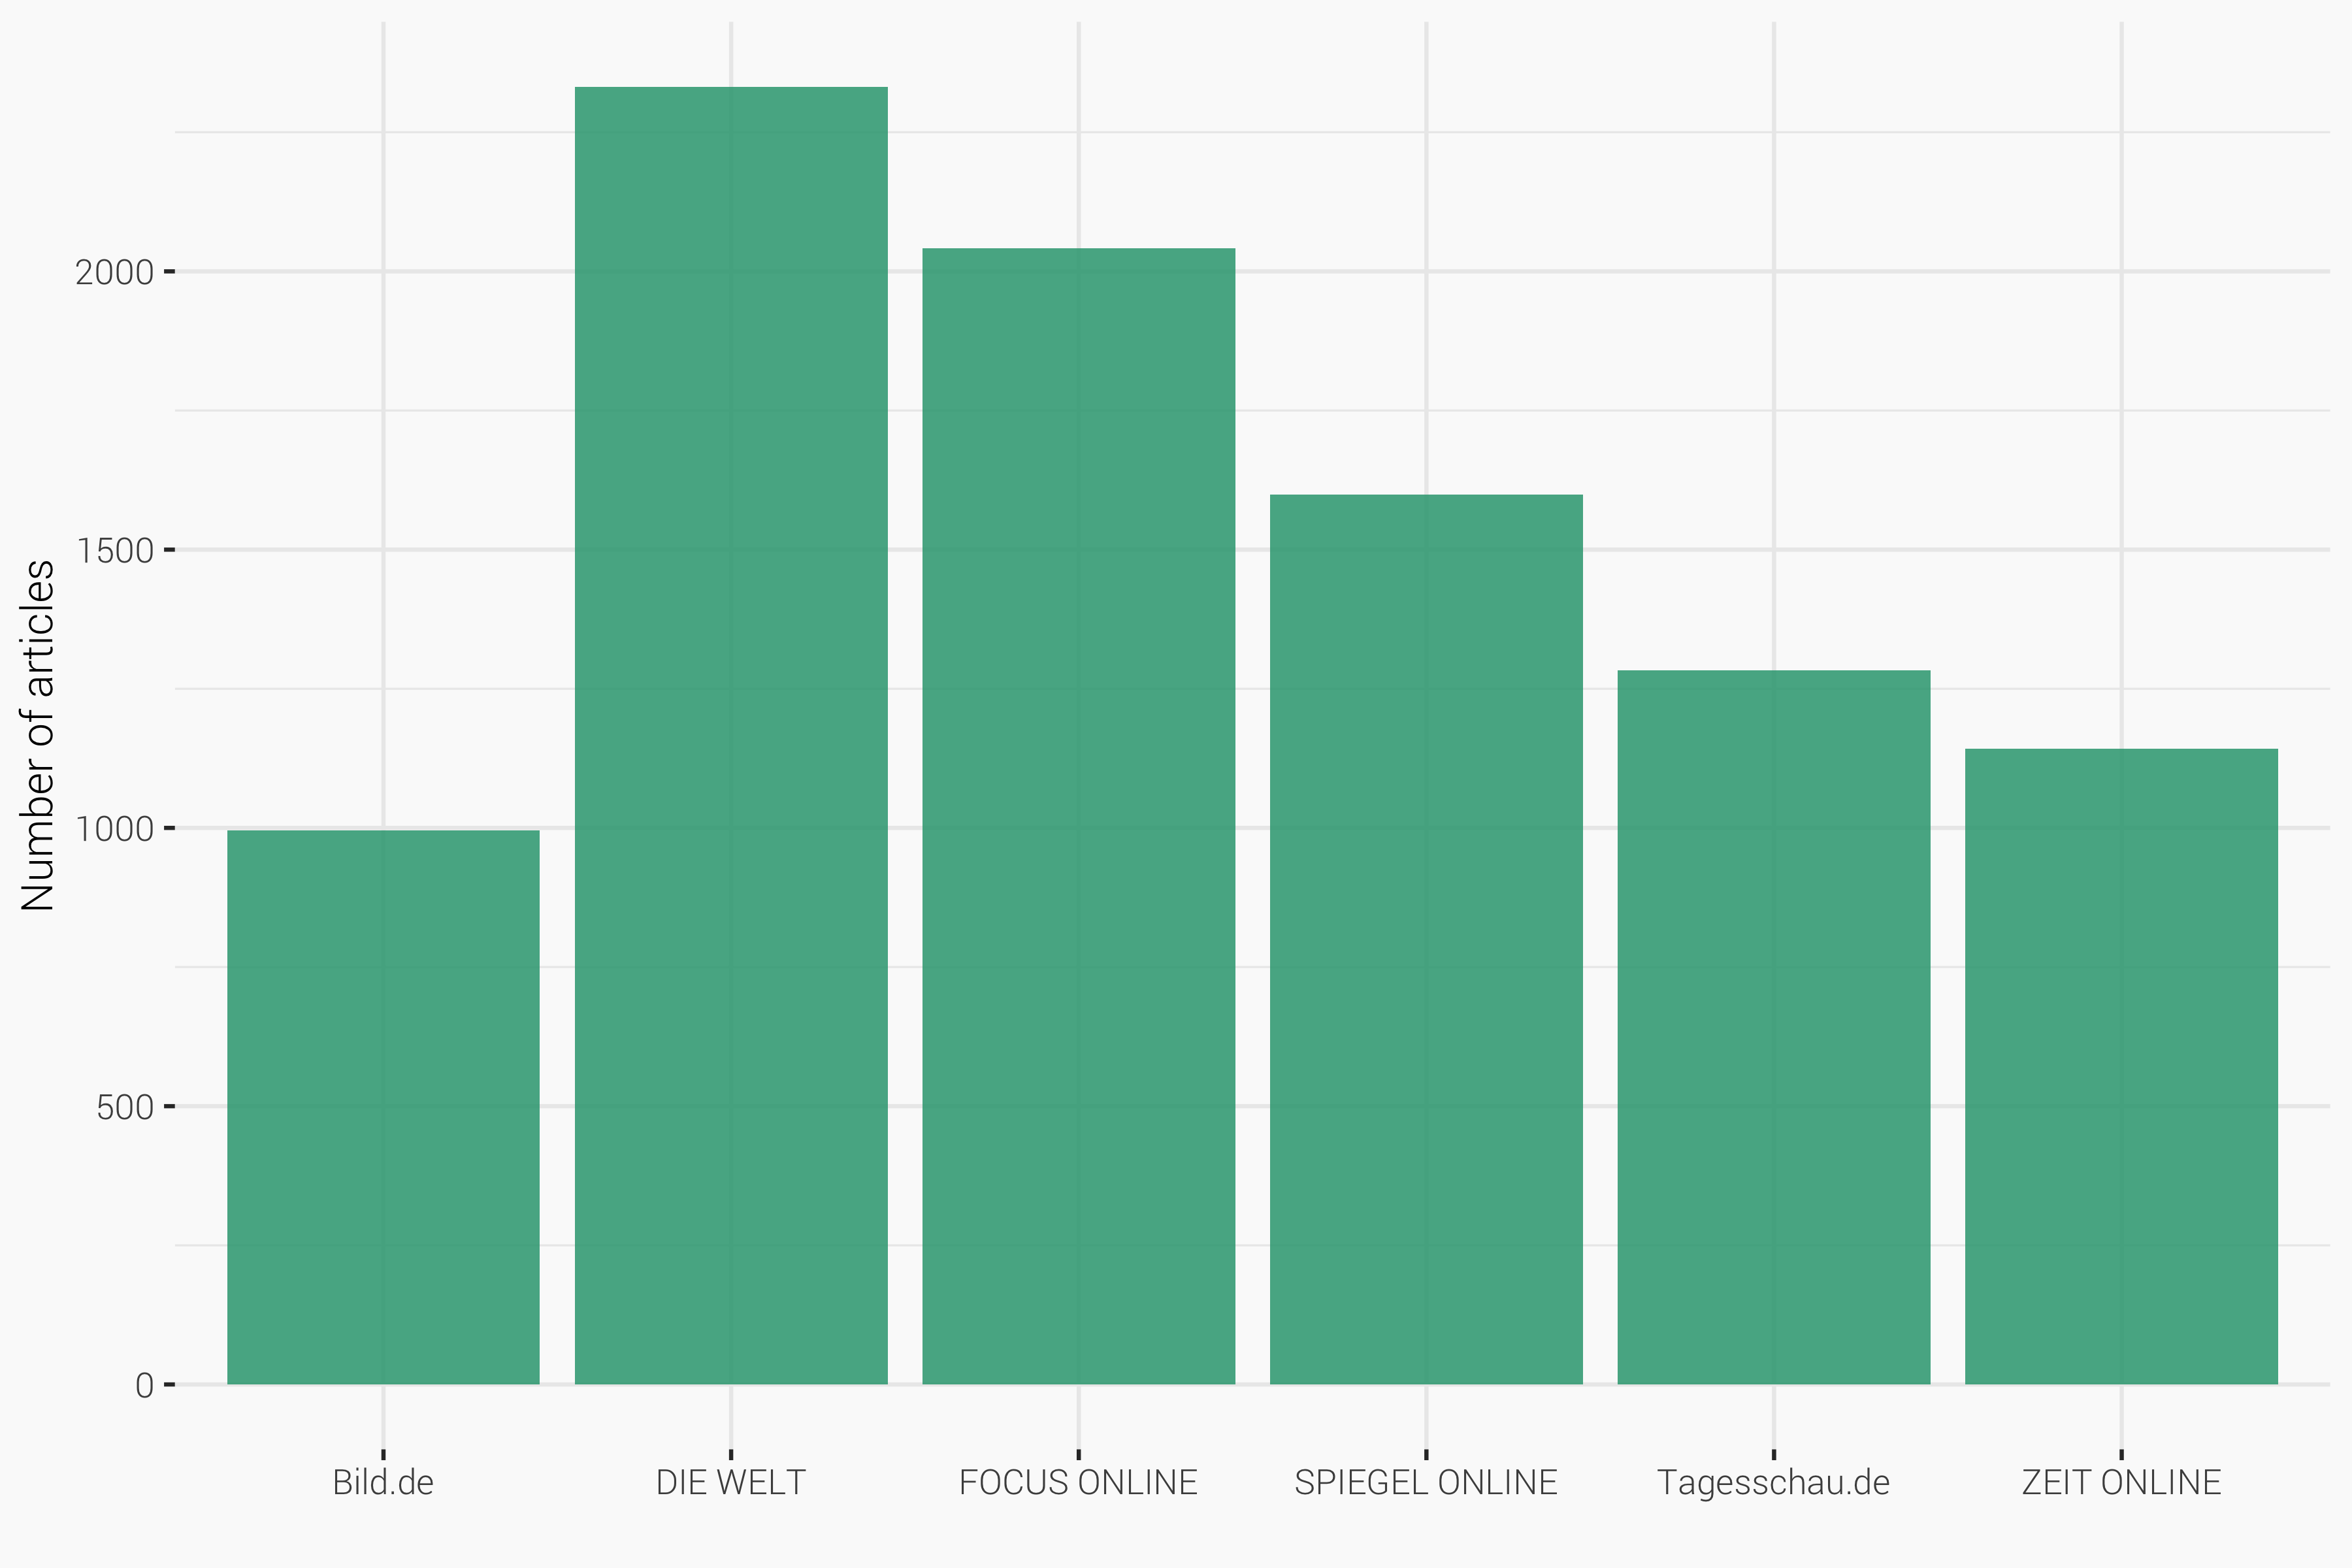
\includegraphics[width=\textwidth]{../figs/bar.png}
			\caption{... by news source}
			\label{fig_distr2}
		\end{subfigure}
	\end{center}
\end{figure}

% ------------------
% Text Pre-Procesing
% ------------------

A central task in text mining is to extract low-dimensional information from documents that are high-dimensional by nature \citep{bholat_text_2015}. This is related to the task of reducing the number of unique language elements in order to reduce the dimensionality of data (to avoid unnecessary computational complexity and overfitting) while at the same time keeping those words that reflect the content of a document. Any useful representation of text will throw away some information, the trick is to include the relevant information for our needs, and exclude the extraneous information. A common strategy to use text as data and reduce the dimensionality, is to pre-process the text by imposing some preliminary restrictions (stop-word removal, tokenization) based on the nature of the data (twitter text, newspaper articles, speeches, etc.) to reduce the number of language elements \citep{gentzkow_text_2017}. Intuitively the term frequency (tf) of a word is a measure of how important that word may be. There are words in a document, however, that occur many times but may not be important like articles, conjunctions, and so on. These terms, often called "stop words", are important to the grammatical structure of a text, but typically don't add any additional meaning and can therefore be neglected. We use a pre-defined stop word list from the Snowball stemmer project\footnote{http://svn.tartarus.org/snowball/trunk/website/algorithms/*/stop.txt} together with a customized list of stop-words that are redundant superfluous or distorting. We also remove punctuation character (e.g. ., ,, !, ?, etc.) and all numbers from our corpus. After completing this steps we were left with 55.235 unique terms in our vocabulary.

After pre-processing, each document $d$ is a finite list of terms. Each unique term in the corpus is indexed by some $v \in \lbrace 1,...,V \rbrace$ where $V$ is the number of unique terms. For each document $d \in \lbrace 1,...,D \rbrace$ we compute the number of occurrences of term $v$ in document $d$ to obtain the count $x_{d,v}$. The $D$ x $V$ matrix $\boldsymbol{X}$ of all such counts is called the document-term matrix. This representation is often referred to as the bag of words model, since the order in which words are used within a document is completely disregarded. 

% ----------------------
% Structural topic Model
% ----------------------
\section{The structural topic model}\label{ch_model}

The structural topic model (STM) developed by \citet{roberts_model_2016} allows to incorporate document specific covariates (e.g. the author or date of a document). STM is a recent extension of the standard topic modeling technique, labeled as "latent Dirichlet allocation" (LDA), which refers to the Bayesian model in \citet{blei_latent_2003} that treats each word in a topic and each topic in a document as generated from a Dirichlet - distributed prior.\footnote{See also \citet{griffiths_probabilistic_2002}, \citet{griffiths_finding_2004} and \citet{hofmann_probabilistic_1999}. \citet{pritchard_inference_2000} introduced the same model in genetics for factorizing gene expression as a function of latent populations.} Topic models formalize the idea that documents are formed by hidden variables (topics) that generate correlations among observed terms. Since its introduction into text analysis, LDA has become hugely popular and especially useful in political science.\footnote{see \citet{blei_probabilistic_2012}, \citet{grimmer_text_2013} and \citet{wiedmann_text_2016} for an overview in social science and \citet{gentzkow_text_2017} give an overview of text mining applications in economics.} \citet{wiedmann_text_2016} uses topic model methods on large amounts of news articles from two german newspapers published between 1959 and 2011, to reveal how democratic demarcation was performed in Germany over the past six decades. \citet{paul_cross-collection_2017} compares editorial differences between media sources, using cross-collection latent Dirichlet allocation (ccLDA), an LDA-based approach that incorporates differences in document metadata. They use a dataset of 623 news articles from August 2008 from two American media outlets - msnbc.com and foxnews.com - to compare how they discuss topics. Reviewing the top words of the word-topic distribution, they find some content differences between the two. 

STM has been applied to multiple academic fields: \citet{roberts_structural_2014} uses STM to analyse open-ended responses from surveys and experiments, \citet{farrell_corporate_2016} applies the model to scientific texts on climate change, revealing links between corporate funding and the framing of scientific studies. \citet{mishler_using_2015} show that "STM can be used to detect significant events such as the downing of Malaysia Air Flight 17" when applied to twitter data. Another study shows how STM can be used to explore the main international development topics of countries’ annual statements in the UN General Debate and examine the country-specific drivers of international development rhetoric \citep{baturo_what_2017}. \citet{mueller_reading_2016} use newspaper text to predict armed conflicts in different regions. They use the estimated topic shares in linear fixed effects regression to forecast conflict out-of-sample. \citet{roberts_navigating_2016} use STM to examine the role of partisanship in topical coverage using a corpus of 13,246 posts that were written for 6 political blogs during the course of the 2008 U.S. presidential election. With the aim of revealing the effect of partisan membership on topic prevalence, each blog is assigned to be either liberal or conservative. To explore the differences between the two, they look at the expected proportion of topic and examine the posts most associated with a respective topic. This approach is similar to \citet{roberts_model_2016}. They also use different measures of distance between the topic-word distributions of the same topic within different models. In section \ref{ch_similarity} a similar approach is applied to measure similarity between the same topic for different covariate levels.

% Topic Modeling
% --------------
\subsection{Generative Process of STM}\label{ch_generativeProcess}

As mentioned above, the STM allows to incorporate observed document metadata which is able to affect both topical prevalence and topical content. The following description of the generative model - the process of filling a word-position in a document - of the STM is based on \citet{roberts_structural_2013} and \citet{roberts_stm:_2016}. For each document $d$ and a given number of topics $K$, a document-specific topic-prevalence vector $d(\boldsymbol{\theta}_d)$ is drawn from a logistic-normal distribution, where the parameters are a function of the covariate values:

\begin{equation}
	\boldsymbol{\theta}_d|\boldsymbol{x}_{d\gamma},\boldsymbol{\Sigma} \sim \textrm{LogisticNormal}(\mu = \boldsymbol{x}_{d\gamma}\boldsymbol{\Sigma}).
\end{equation}

$\boldsymbol{x}_d\gamma$ lists the values of all metadata covariates for document $d$, where $\gamma$ relates these covariate values to the topic-prevalence. The structure of $\boldsymbol{\Sigma}$ implies the possibility of correlations across documents in the topic-prevalence vector. 

According to $\theta$, a specific topic $z_{dn}$ is assigned for the $n^{th}$ word-position in the document through the process:

\begin{equation}
	z_{dn}|\boldsymbol{\theta}_d \sim \textrm{Multinomial}(\boldsymbol{\theta}_d).
\end{equation}

Conditional in the topic chosen, a specific word, $w_{dn}$, is chosen from the overall corpus vocabulary $V$, using the following process:

\begin{equation}
	w_{dn}|z_{dn},\beta_{dkv} \sim \textrm{Multinomial}(\beta_{dk1},...,\beta_{dkV}),
\end{equation}

where the word probability $\beta_{dkv}$ is parameterized in terms of log-transformed rate deviations from the rates of a corpus-wide background distribution $m_v$. The log-transformed rate deviations can then be specified by a collection of parameters $\lbrace \boldsymbol{\kappa} \rbrace$, where $\kappa^{(t)}$ is a $K$-by-$V$ matrix containing the log-transformed rate deviations for each topic $k$ and term $v$, over the baseline log-transformed rate for term $v$. This matrix is the same for all $A$ levels of covariates. To put it differently, $\kappa^{(t)}$ indicates the importance of the term $v$ given topic $k$ regardless of the covariates. Similarly, $\kappa^{(c)}$ is a $A$-by-$V$ matrix, indicating the importance of the term $v$ given the covariate level $c$ regardless of the topic. Finally, $\kappa^{(i)}$ is a $A$-by-$K$-by-$V$ matrix, collecting the covariate-topic effects:

\begin{equation}
	\beta_{dkv}|z_{dn}=\frac{\textrm{exp}(m_v+\kappa^{(t)}_{kv},\kappa^{(c)}_{y_dv}+\kappa^{(i)}_{y_dkv})}{\sum_v \textrm{exp}(m_v+\kappa^{(t)}_{kv},\kappa^{(c)}_{y_dv}+\kappa^{(i)}_{y_dkv})}.
\end{equation}

The STM maximizes the posterior likelihood that the observed data were generated by the above data-generating process using an iterative approximation-based variational expectation-maximization algorithm\footnote{A technical description of this maximization process can be found in \citet{roberts_model_2016}} available in R's stm package \citep{roberts_stm:_2016}. The process gives us two posterior distribution parameter: (1) $\beta$ is a $K$-by-$V$ matrix (where $K=$ number of topics and $V=$ vocabulary), where the entry $\beta_{kvc}$ can be interpreted as the probability of observing the $v$-th word in topic $k$ for the covariate level $c$. (2) $\theta$ is a $D$-by-$V$ matrix of the document-topic distributions, where the entry $\theta_{dk}$ can be interpreted as the proportion of words in document $d$ which arise from topic $k$, or rather as the probability that document $d$ deals about topic $k$. These probability distributions are used to compare the content of public and private news providers in section \ref{ch_empirical}.


% ----------------------
% Model Selection
% ----------------------
\subsection{Model and parameter selection}

Inference of mixed-membership models, such as the one applied in this paper, has been a thread of research in applied statistics in the past few years \citep{blei_latent_2003} \citep{erosheva_mixed-membership_2004} \citep{braun_variational_2010}. Topic models are usually imprecise as the function to be optimized has multiple modes, such that the model results can be sensitive to the starting values. Since an ex ante valuation of a model is hardly possible, I compute a variety of different models and compare their posterior probability. This enables me to check how results vary for different model solution \citep{roberts_navigating_2016}. I then cross-checked some subset of assigned topic distributions to evaluate whether the estimates align with the concept of interest \citep{gentzkow_text_2017}. These manual audits are applied together with numeric optimization based on the topic coherence measure suggested by \citet{mimno_optimizing_2011}. 

This process revealed that a model with 50 topics best reflects the structure in the corpus. Furthermore, the publisher of the article is used as covariates in the topic prevalence and topical content. In other words, the corresponding newswire of an article influences the probability distribution of topics and how the topics are discussed. To address problems due to non-convexity, we rely on the spectral initialization approach advocated by \citet{roberts_navigating_2016}. 

% ----------------------
% Model Results
% ----------------------
\section{Empirical Evaluation}\label{ch_empirical}

This section summarizes the results of the STM. Subsequently "the two T's" (Topic and Tone) of the corpus are analyzed according to the following approaches: (1) The document-topic probability $\theta$ is used, to estimate the conditional expectation of topic prevalence for given document characteristics (See section \ref{subsection_topic}). A set of topics is selected, that most distinctly discuss a particular party (or a topic related to a party). (2) Articles that are assigned to the selected topics with the highest probability are then used to conduct a dictionary-based analysis (see section \ref{subsection_tone}). 

\subsection{Topic}\label{subsection_topic}

In order to get an initial overview of the results, Figure \ref{fig_topic_proportion} displays the topics ordered by their expected frequency across the corpus (left side of the Figure) and the expected proportion of a topic in public media minus the expected proportion of topic use in private media (right side of the Figure). Thus topics more associated with public media appear to the right of zero. To assign a label to each topic, I looked at the most frequent words in that topic and the most representative articles \citep{roberts_model_2016}. 

It becomes apparent that the topic (topic 4) about the coalition talks between CDU/CSU and SPD - the "Great coalition" or "GroKo" (from the German word Große Koalition) - is the topic with the highest expected frequency in the whole corpus, followed by the topic about the so-called Jamaica parties (CDU/CSU, FDP and Bündnis 90/Die Grünen), which was the first alternative to be negotiated directly after the elections. The Figure also shows, that topics related to refugees in Germany (topics 12 and 42) are quite frequent within the corpus. We will select the following topics from the whole set (topic are ordered regarding their overall corpus frequency):

\begin{enumerate}
	\item Topic 4: Covering the debates about the great coalition talks, mainly after the failure of the Jamaica coalition talks. 
	\item Topic 27: Covering the Jamaica coalition talks, mainly focusing on the smaller players Bündnis 90/Die Grünen and FDP.
	\item Topic 23: About issues regarding the CSU, mainly about the competition between Horst Seehofer and Markus Söder and the negotiations with the CDU.
	\item Topic 37: Covering debates of AfD and DIE LINKE in the parliament (Deutscher Bundestag).
	\item Topic 17: Covering votes within the SPD, mainly regarding the vote about a possible coalition with CDU/CSU ("GroKo")
	\item Topic 26: Discussing the failure of the Jamaica coalition talks and the two possible alternatives: Reelections or a great coalition.
	\item Topic 13: About Angela Merkel, mainly right before the election.
	\item Topic 1: About the SPD, mainly about the election campaign and Martin Schulz as candidate for the chancellor.
	\item Topic 32: About the AfD, mainly about Alice Weidel and Alexander Gauland, voted as parliamentary party leaders after the resignation of Frauke Petry.
	\item Topic 30: About the AfD, mainly about the resignation of Frauke Petry and Jörg Meuthen.
	\item Topic 2: About Bündnis 90/Die Grünen, mainly covering issues regarding the party's personell debates.
	\item Topic 22: About SPD, mainly covering issues regarding the party's personell debates
	\item Topic 20: About the AfD, mainly about their relation to right-wing extremist groups.
	\item Topic 46: Covering issues regarding the CDU.
\end{enumerate}   

\begin{figure}[H]
	\begin{center}
	\caption{Expected topic proportion}
		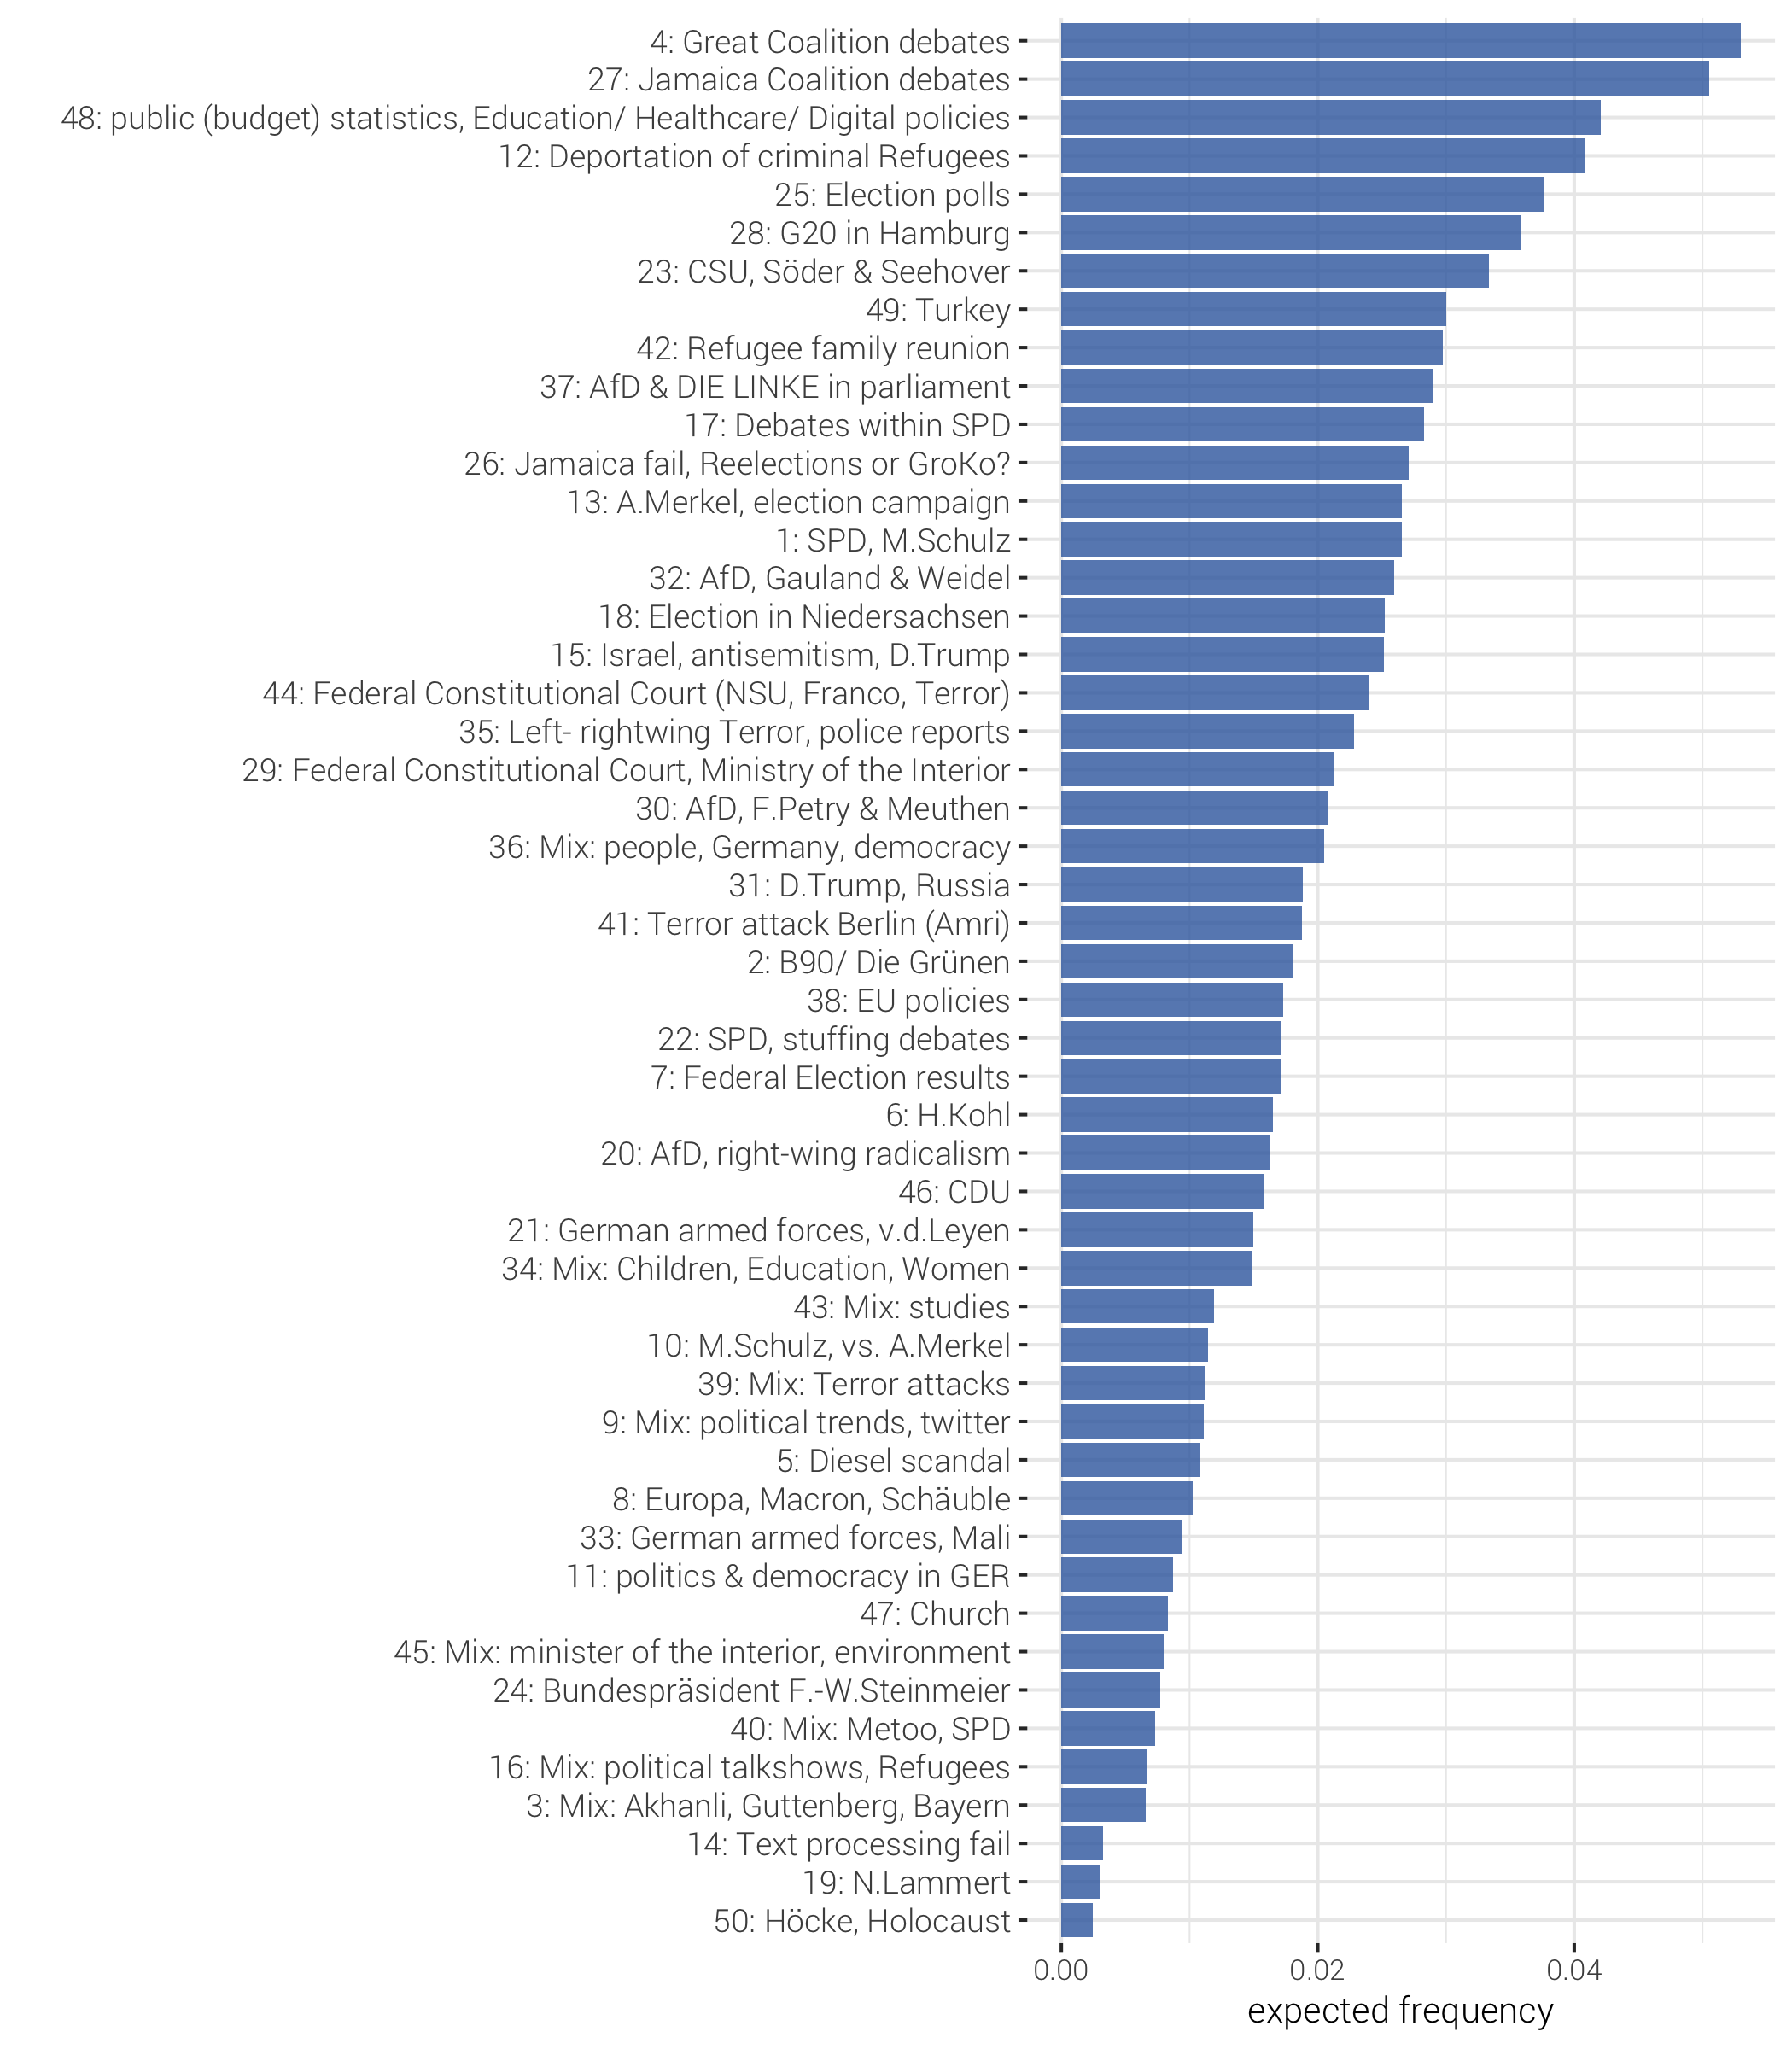
\includegraphics[width=\textwidth,keepaspectratio]{../figs/topic_proportion.png}
		\label{fig_topic_proportion}
\end{center}
\end{figure}

Next, the differences of topic prevalence for given document characteristics can be estimated \citep{roberts_model_2016}. More specifically, I estimate a linear model, where the documents are observations, the dependent variable is the posterior probability of a topic and the covariates are the metadata of documents (see equation \ref{eq_1}). The stm-package provides a function that uses the method of composition to incorporate uncertainty in the dependent variable, drawing a set of topic proportions from the variational posterior repeated times and compute the coefficients as the average over all results \citep{roberts_stm:_2016}.

\begin{equation}\label{eq_1}
	\theta_d=\alpha+\beta x_{ownership}+\epsilon
\end{equation}

Figure \ref{fig_estimateEffects} shows the regression results for the above selected topics. The coefficients indicate the deviation from the base value of Bild.de.  

\begin{figure}[H]
	\caption{Regression results}
		\begin{center}
			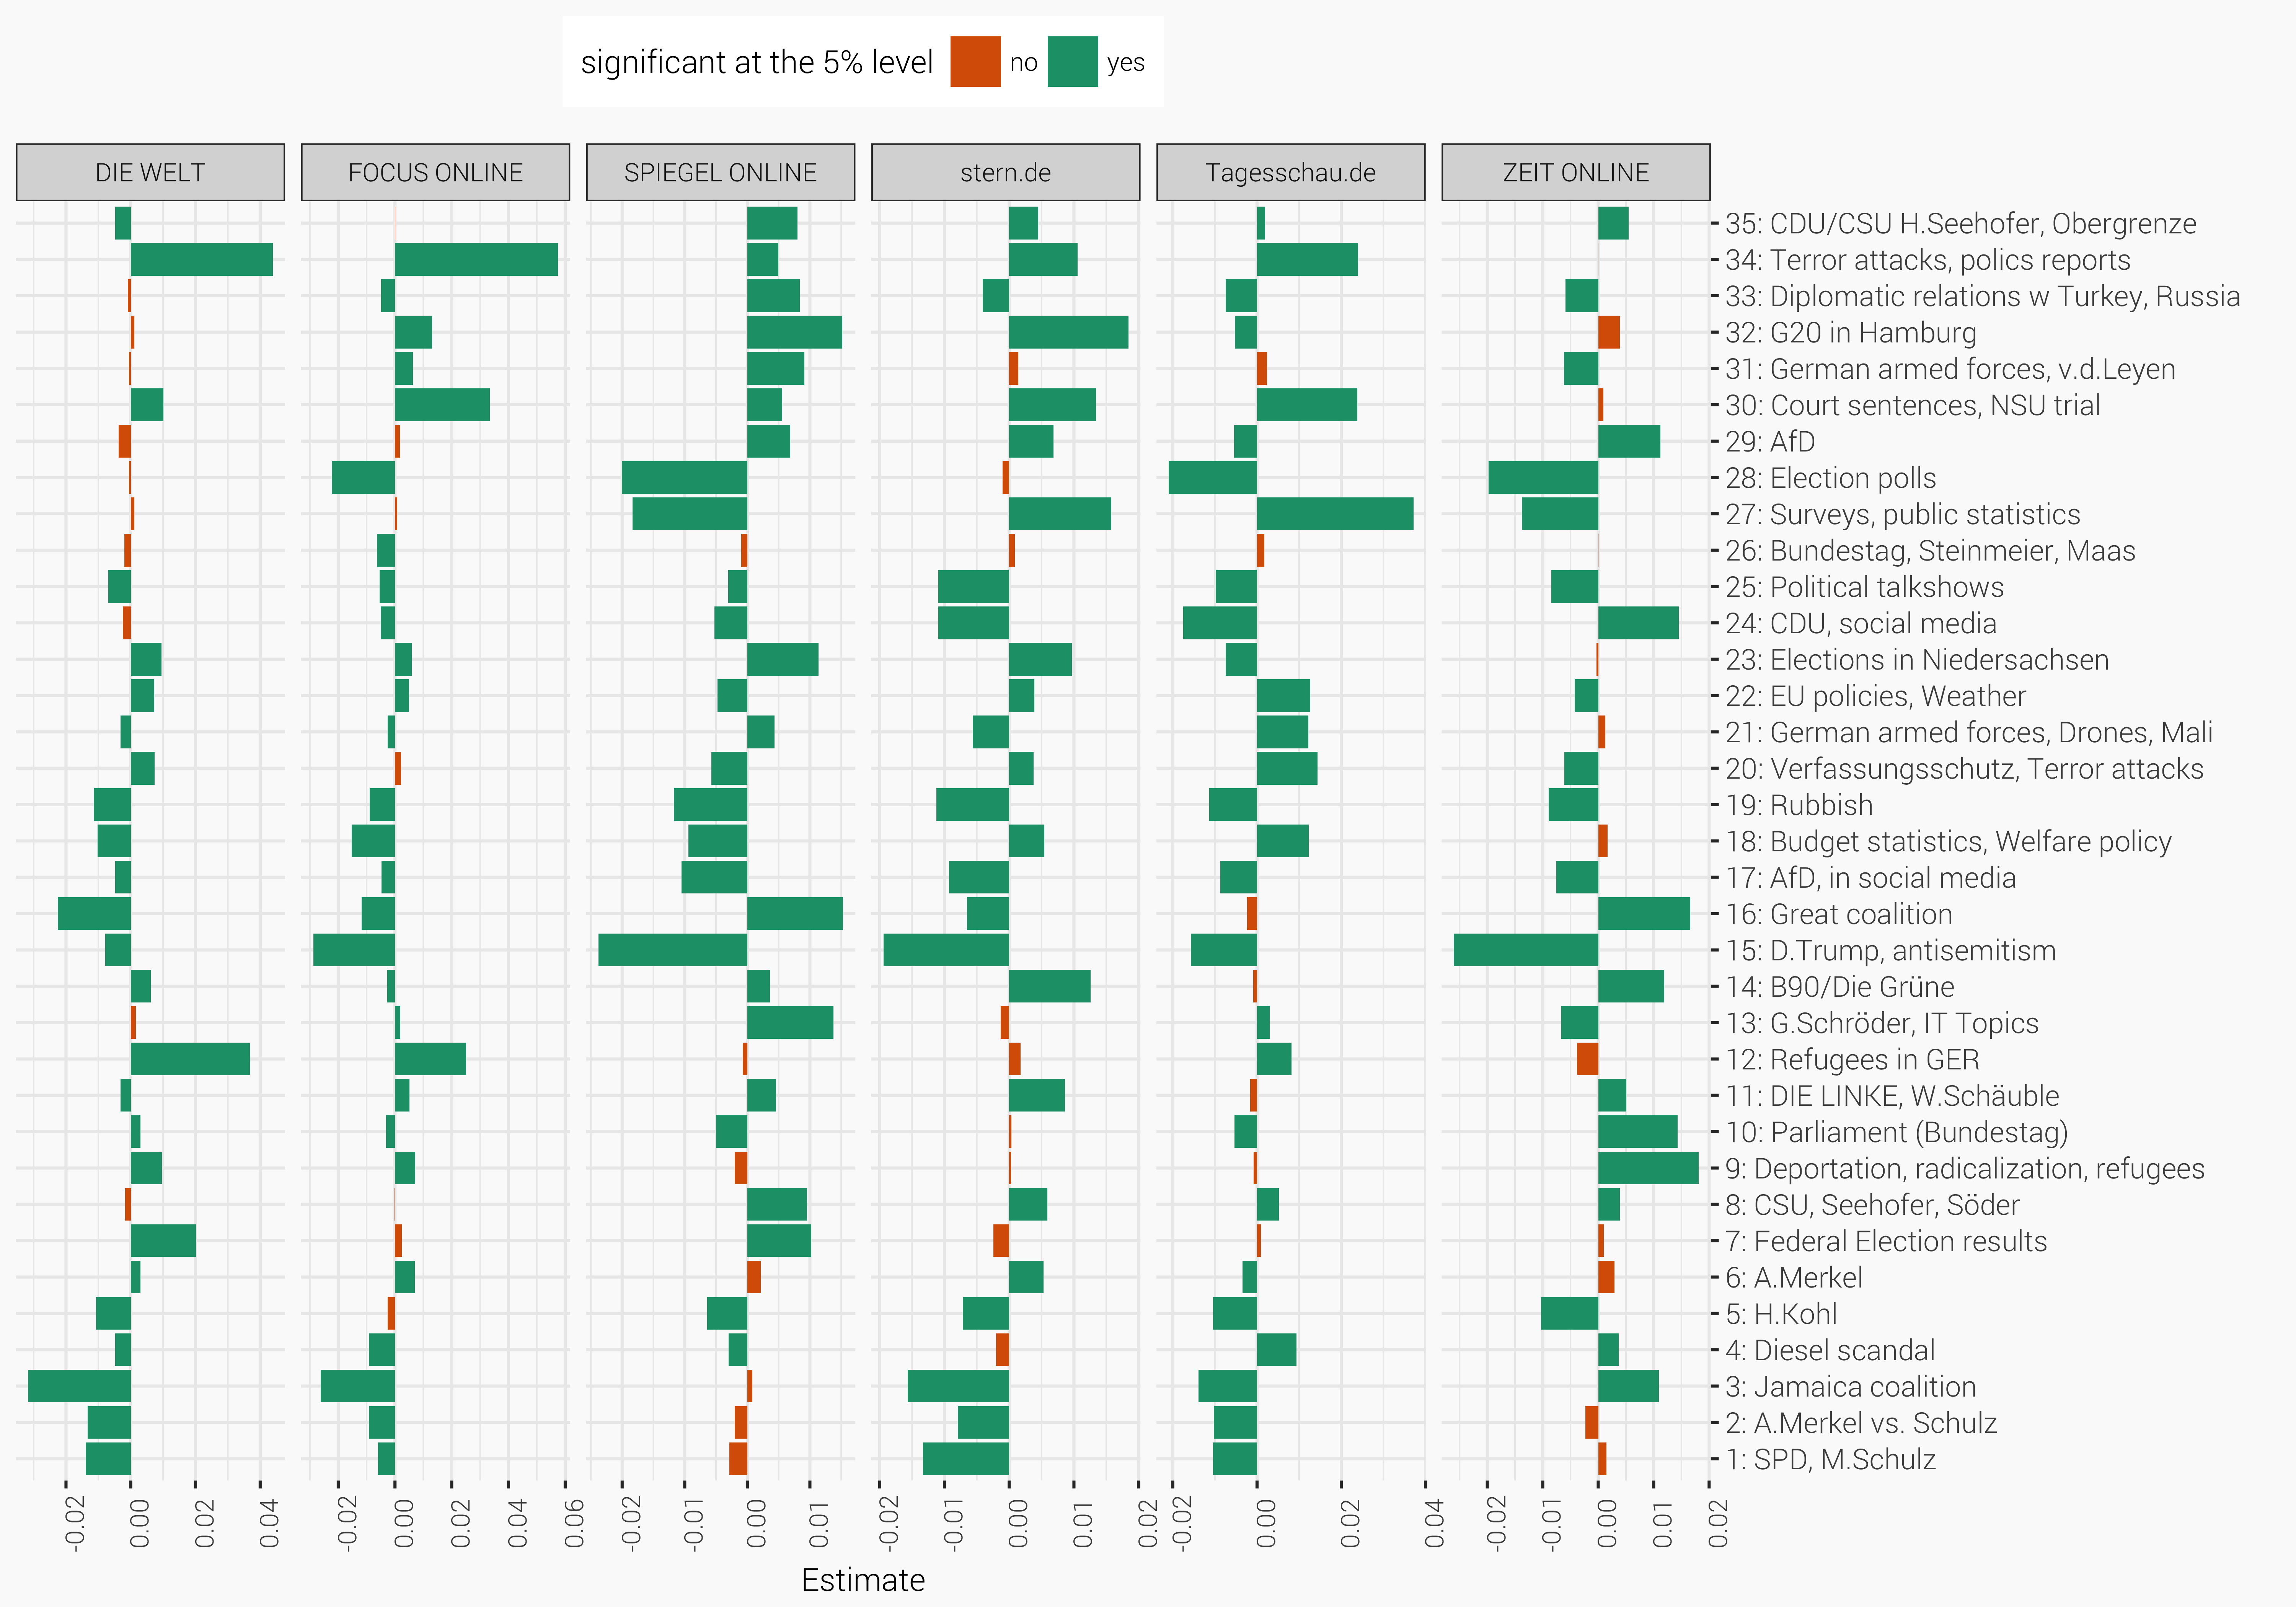
\includegraphics[width=\textwidth,keepaspectratio]{../figs/estimates.png}
		\end{center}
	\label{fig_estimateEffects}
\end{figure}

\textcolor{red}{AUSWERTUNG}


\subsection{Tone}\label{subsection_tone}

Once we identifying the topics of interest, we use only these documents that are assigned to one of the topics with the highest probability. A dictionary-based method is then applied on the remaining 5611 documents with the aim to measure the tone (or sentiment) of a document. The idea of a sentiment analysis is to determine the attitude of a writer toward the overall tonality of a document. To conduct such an analysis, a lists of words (dictionary) associated with a given emotion, such as negativity is pre-defined by the analyst. The document is then deconstructed into individual words and the frequencies of words contained in a given dictionary are then calculated. 

Such lexical or “bag-of-words” approaches are widely presented in the finance literature to  determine  the  effect  of  central  banks’  monetary  policy  communications on asset prices and real variables (\citet{nyman_news_2018} \citep{tetlock_giving_2007}, \citep{tetlock_more_2008}). \citet{hansen_shocking_2016} use a similar approach to measure "the two Ts" (Topic and tone). They explore the effects of FOMC statements on both market and real economic variables. To understand the multi-dimensional information a statement is transmitting, they apply LDA on a corpus of 142 FOMC decision statements split into sentences (topic). They then measure how the central bank is talking about that topic, using a dictionary approach (tone). To calculate their score, they subtract the negative words from the positive words und divide this by the number of total words of the statement. A similar score is used by \citet{nyman_news_2018}, who measure the effect of narratives and sentiment of financial market text-based data on developments in the financial system. They count the number of occurrences of excitement words and anxiety words and then scale these numbers by the total text size as measured by the number of characters.

The present paper uses a dictionary that lists words associated with positive and negative polarity weighted within the interval of $[-1; 1]$. SentimentWortschatz\footnote{SentiWS for short. available here: http://wortschatz.uni-leipzig.de/de/download}, is a publicly available German-language resource for sentiment analysis, opinion mining etc. The current version of SentiWS (v1.8b) contains 1,650 positive and 1,818 negative words, which sum up to 15,649 positive and 15,632 negative word forms incl. their inflections, respectively. The sentiment score for each document $d$ is calculated  based on the weighted polarity values for a word, defined on an interval between -1 and 1. The score is then calculated from the sum of the words in a document (which can be assigned to a word from the dictionary) divided by the total number of words in that document:
 
\begin{equation}
	\text{SentScore}_d = \frac{|\text{positive polarity score}_d| - |\text{negative polarity score}_d|}{|\text{TotalWords}_d|}
\end{equation}

The following figure shows the results of the analysis for each topic on a monthly basis, aggregated on all newspaper. Each sentiment value is weighted by the relative share of the topic in the overall reporting of that month.

Some conclusions can be drawn from this illustration. First of all, it can be seen that, on average, all topics are discussed almost exclusively negatively. An exception is topic 27 concerning the Jaimaica coalition negotiations, which shows a positive sentiment value for a short period of time (October 2017). In the following month (November 2017), after it became clear that there would be no coalition between the CDU/CSU, FDP and Die Grünen, the value of this topic as well as that of topic 26 drops rapidly. 

Concerning the issues that discuss the great coalition between CDU/CSU and SPD, it is evident that the overall tone is in which this topic is discussed is generally decreasing from November 2017 to January 2018, but in the following February, the sentiment value of this topic rises. However, the sentiment score of topics that deal with the SPD alone (1, 17, 22) is diminishing in the course of time, with topic 17 recording the largest decline. The topic, which contains the CDU in isolation (46), is rather zigzagging, with a low peak in October 2017.

If aggregated by news provider, some differences between the sites are discernible (Figure \ref{fig_sentscore_site}). To begin with, it should be noted that on average all topics are discussed negatively by all news providers, except topic 22, which mainly covers the personnel debates of the SPD and has a positive value at Tagesschau.de. One striking feature is the way in which the Jamaica negotiations are reported. Although all providers discuss this topic in a negative light, Bild.de reports this topic particularly negative. The same applies to the reports on the grand coalition, where the value of ZEIT ONLINE is the most negative. A good overview of how differently the topics are discussed by the providers is also shown in Figure \ref{fig_sentscore_radar}. This also clearly shows that the sentiment value of the media differs most notably with regard to topic 27 and topic 4, i. e. the topics on which the coalition negotiations are reported. Furthermore, it becomes evident that the negative sentiment value of FOCUS ONLINE regarding topic 17 is high in relation to the other media. FOCUS ONLINE thus reports comparatively more negatively on the debates within the SPD. This includes in particular the vote on a possible coalition with CDU/CSU. For topic 1, which also deals with the SPD, the value of FOCUS ONLINE is rather negative, only undercut by Bild.de.

\begin{figure}[H]
	\caption{Monthly Sentiment Score}
		\begin{center}
			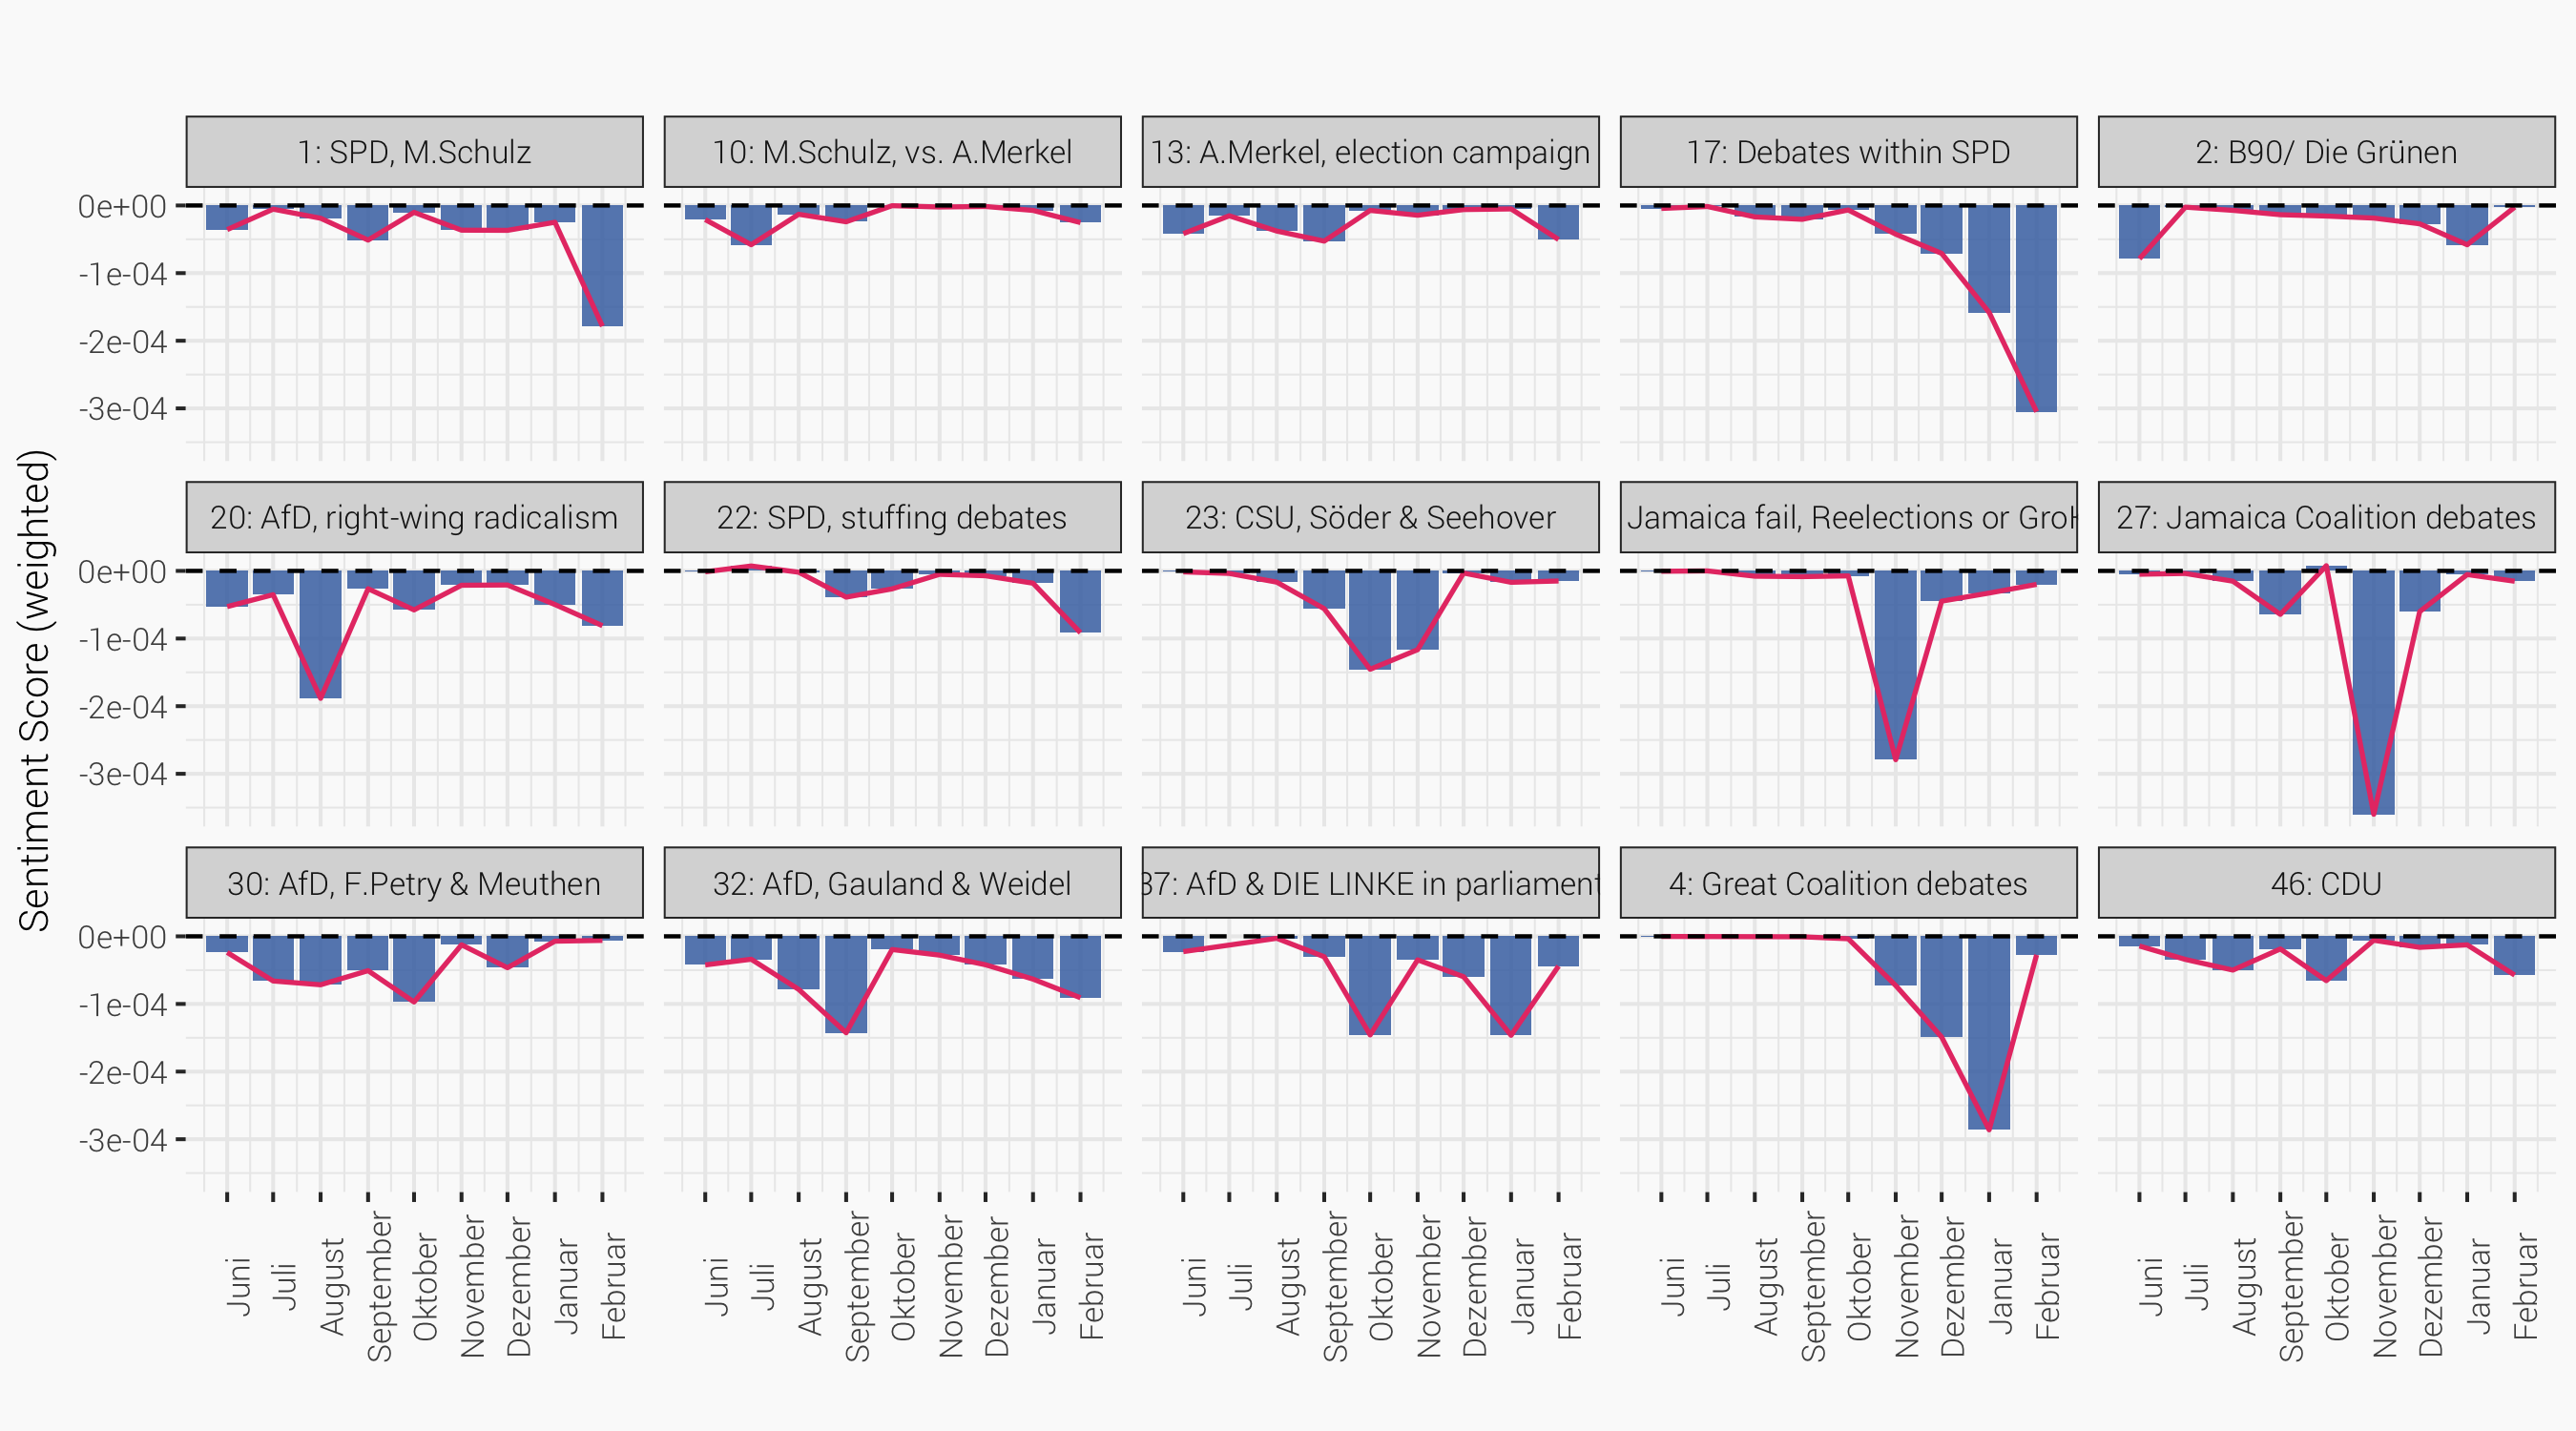
\includegraphics[width=\textwidth,keepaspectratio]{../figs/sentscore_monthly.png}
		\end{center}
	\label{fig_sentscore_monthly}
\end{figure}

\begin{figure}[H]
	\caption{Sentiment Score by news wire}
	\begin{center}
		\begin{subfigure}[normla]{\textwidth}
			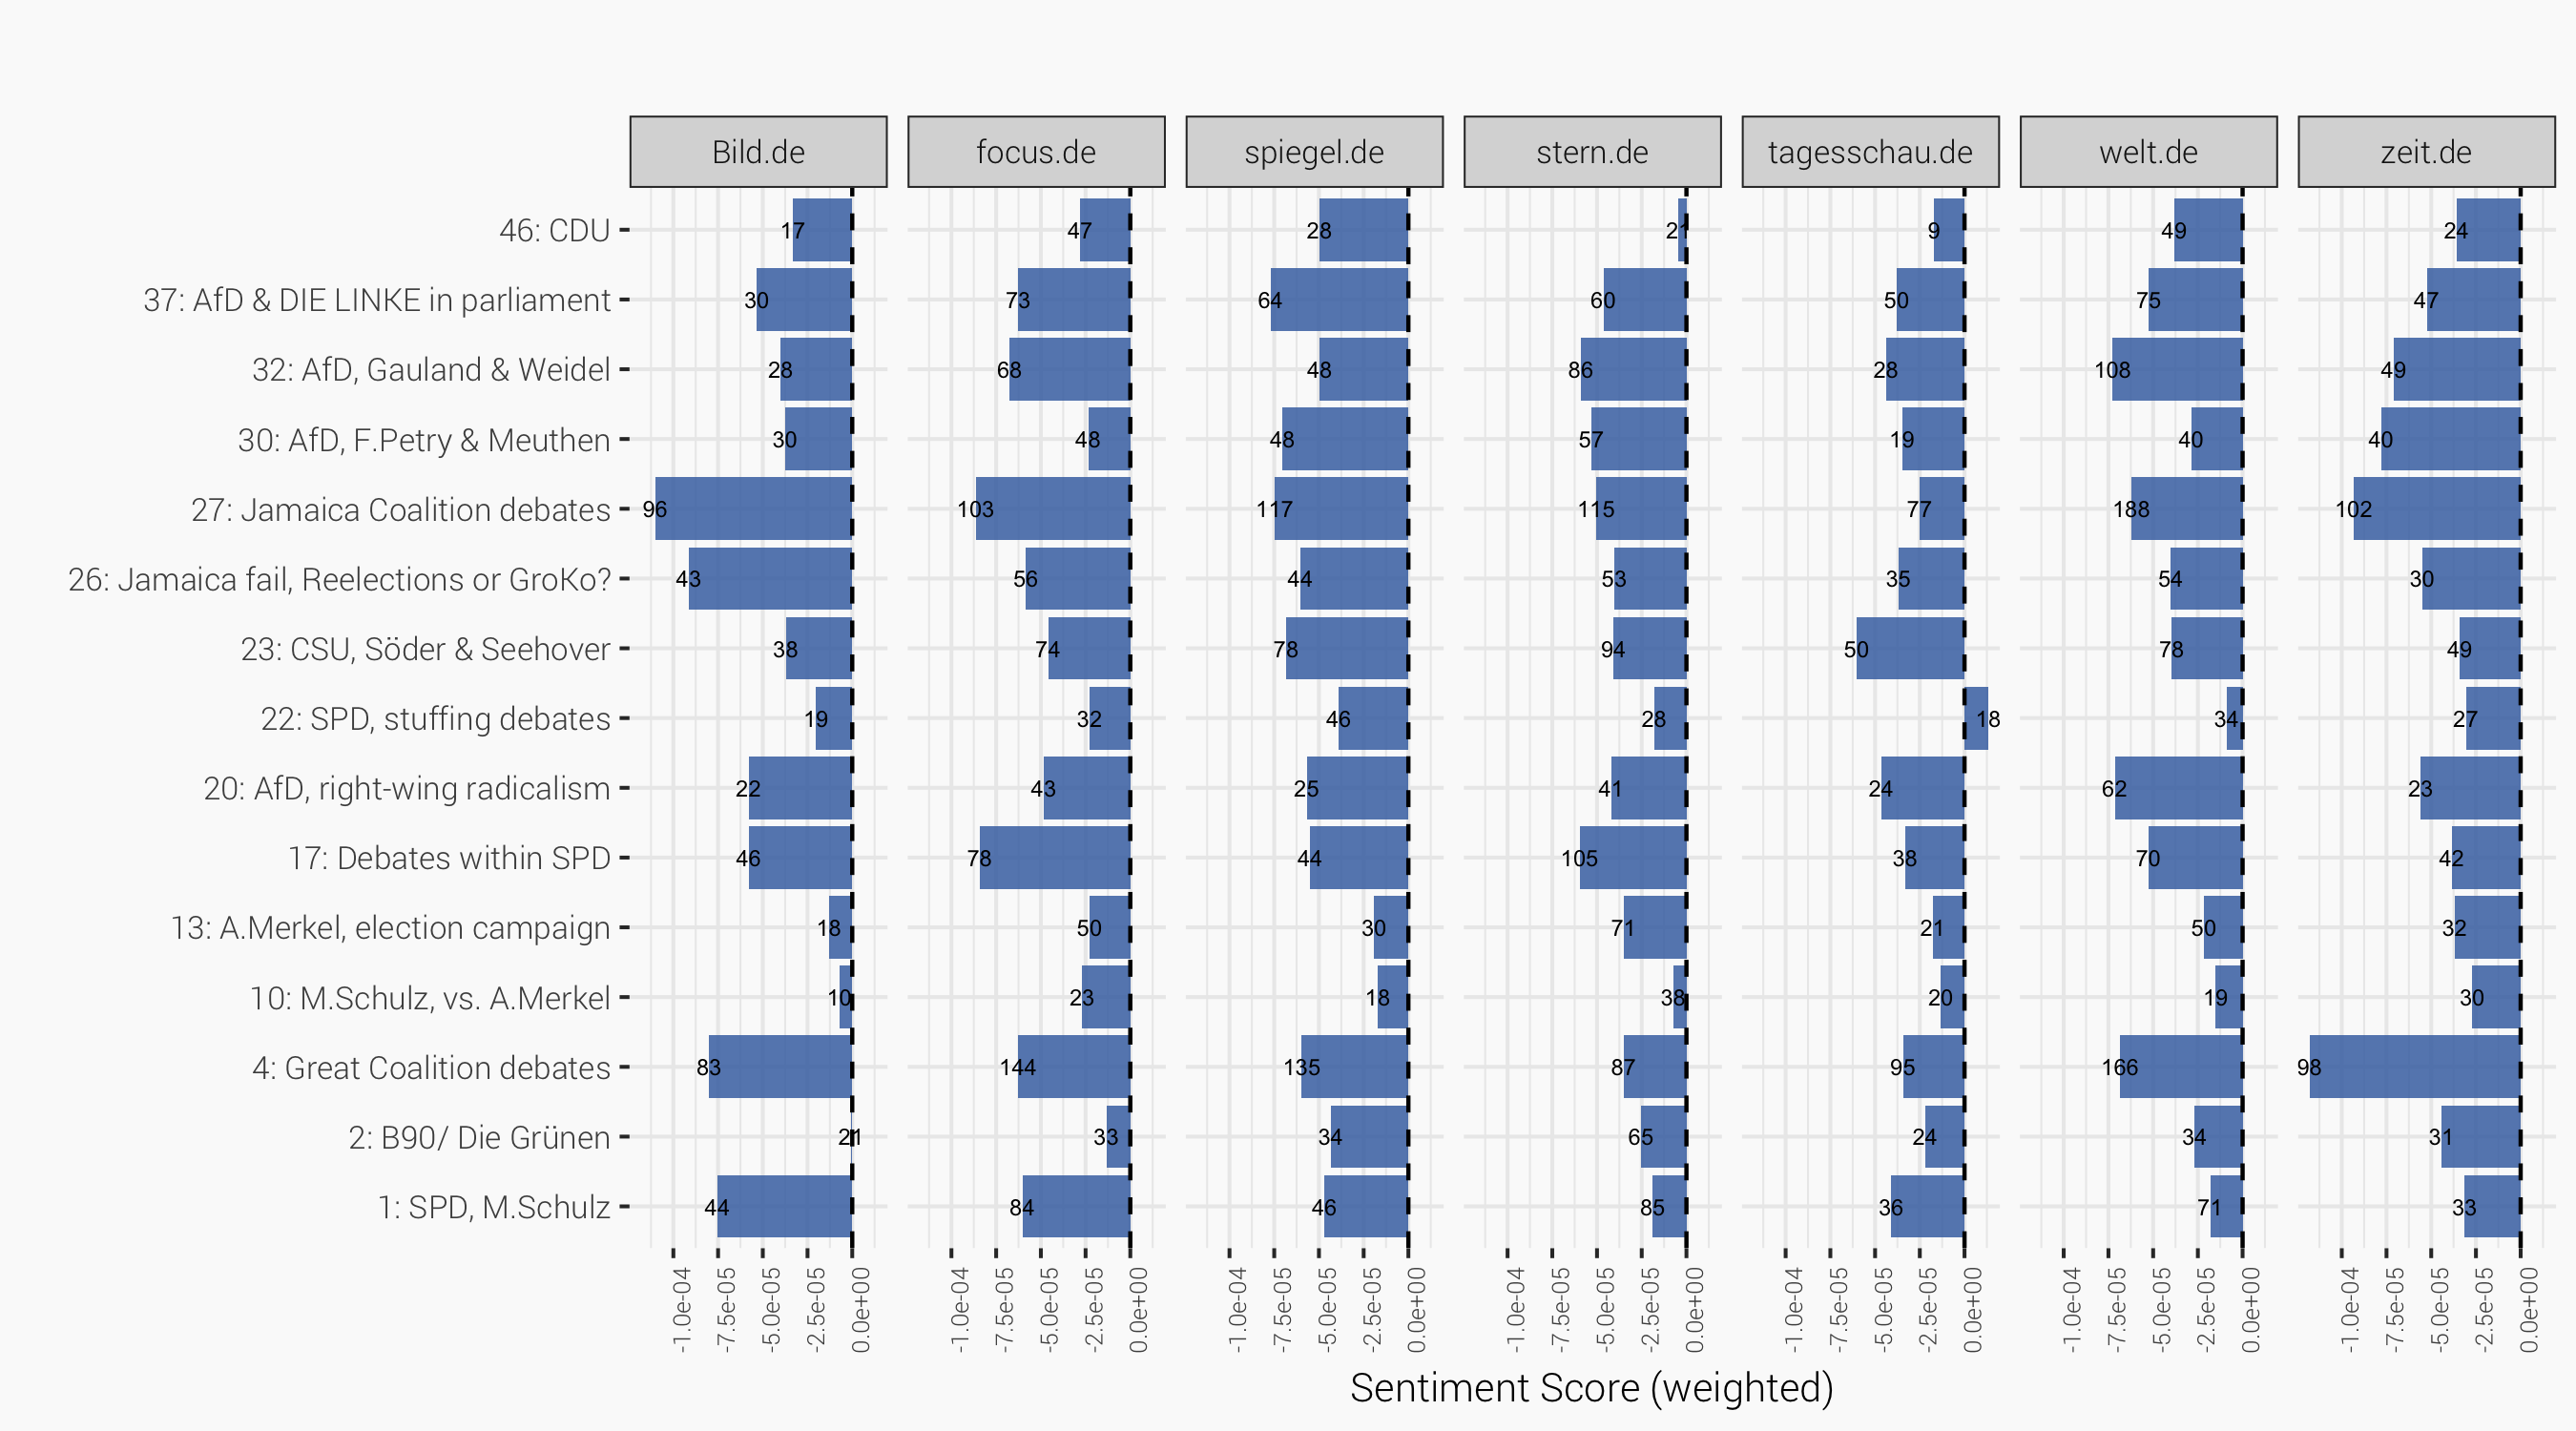
\includegraphics[width=\textwidth,keepaspectratio]{../figs/sentscore_site.png}
			\label{fig_sentscore_site}
		\end{subfigure}
		\begin{subfigure}[normla]{0.7\textwidth}
			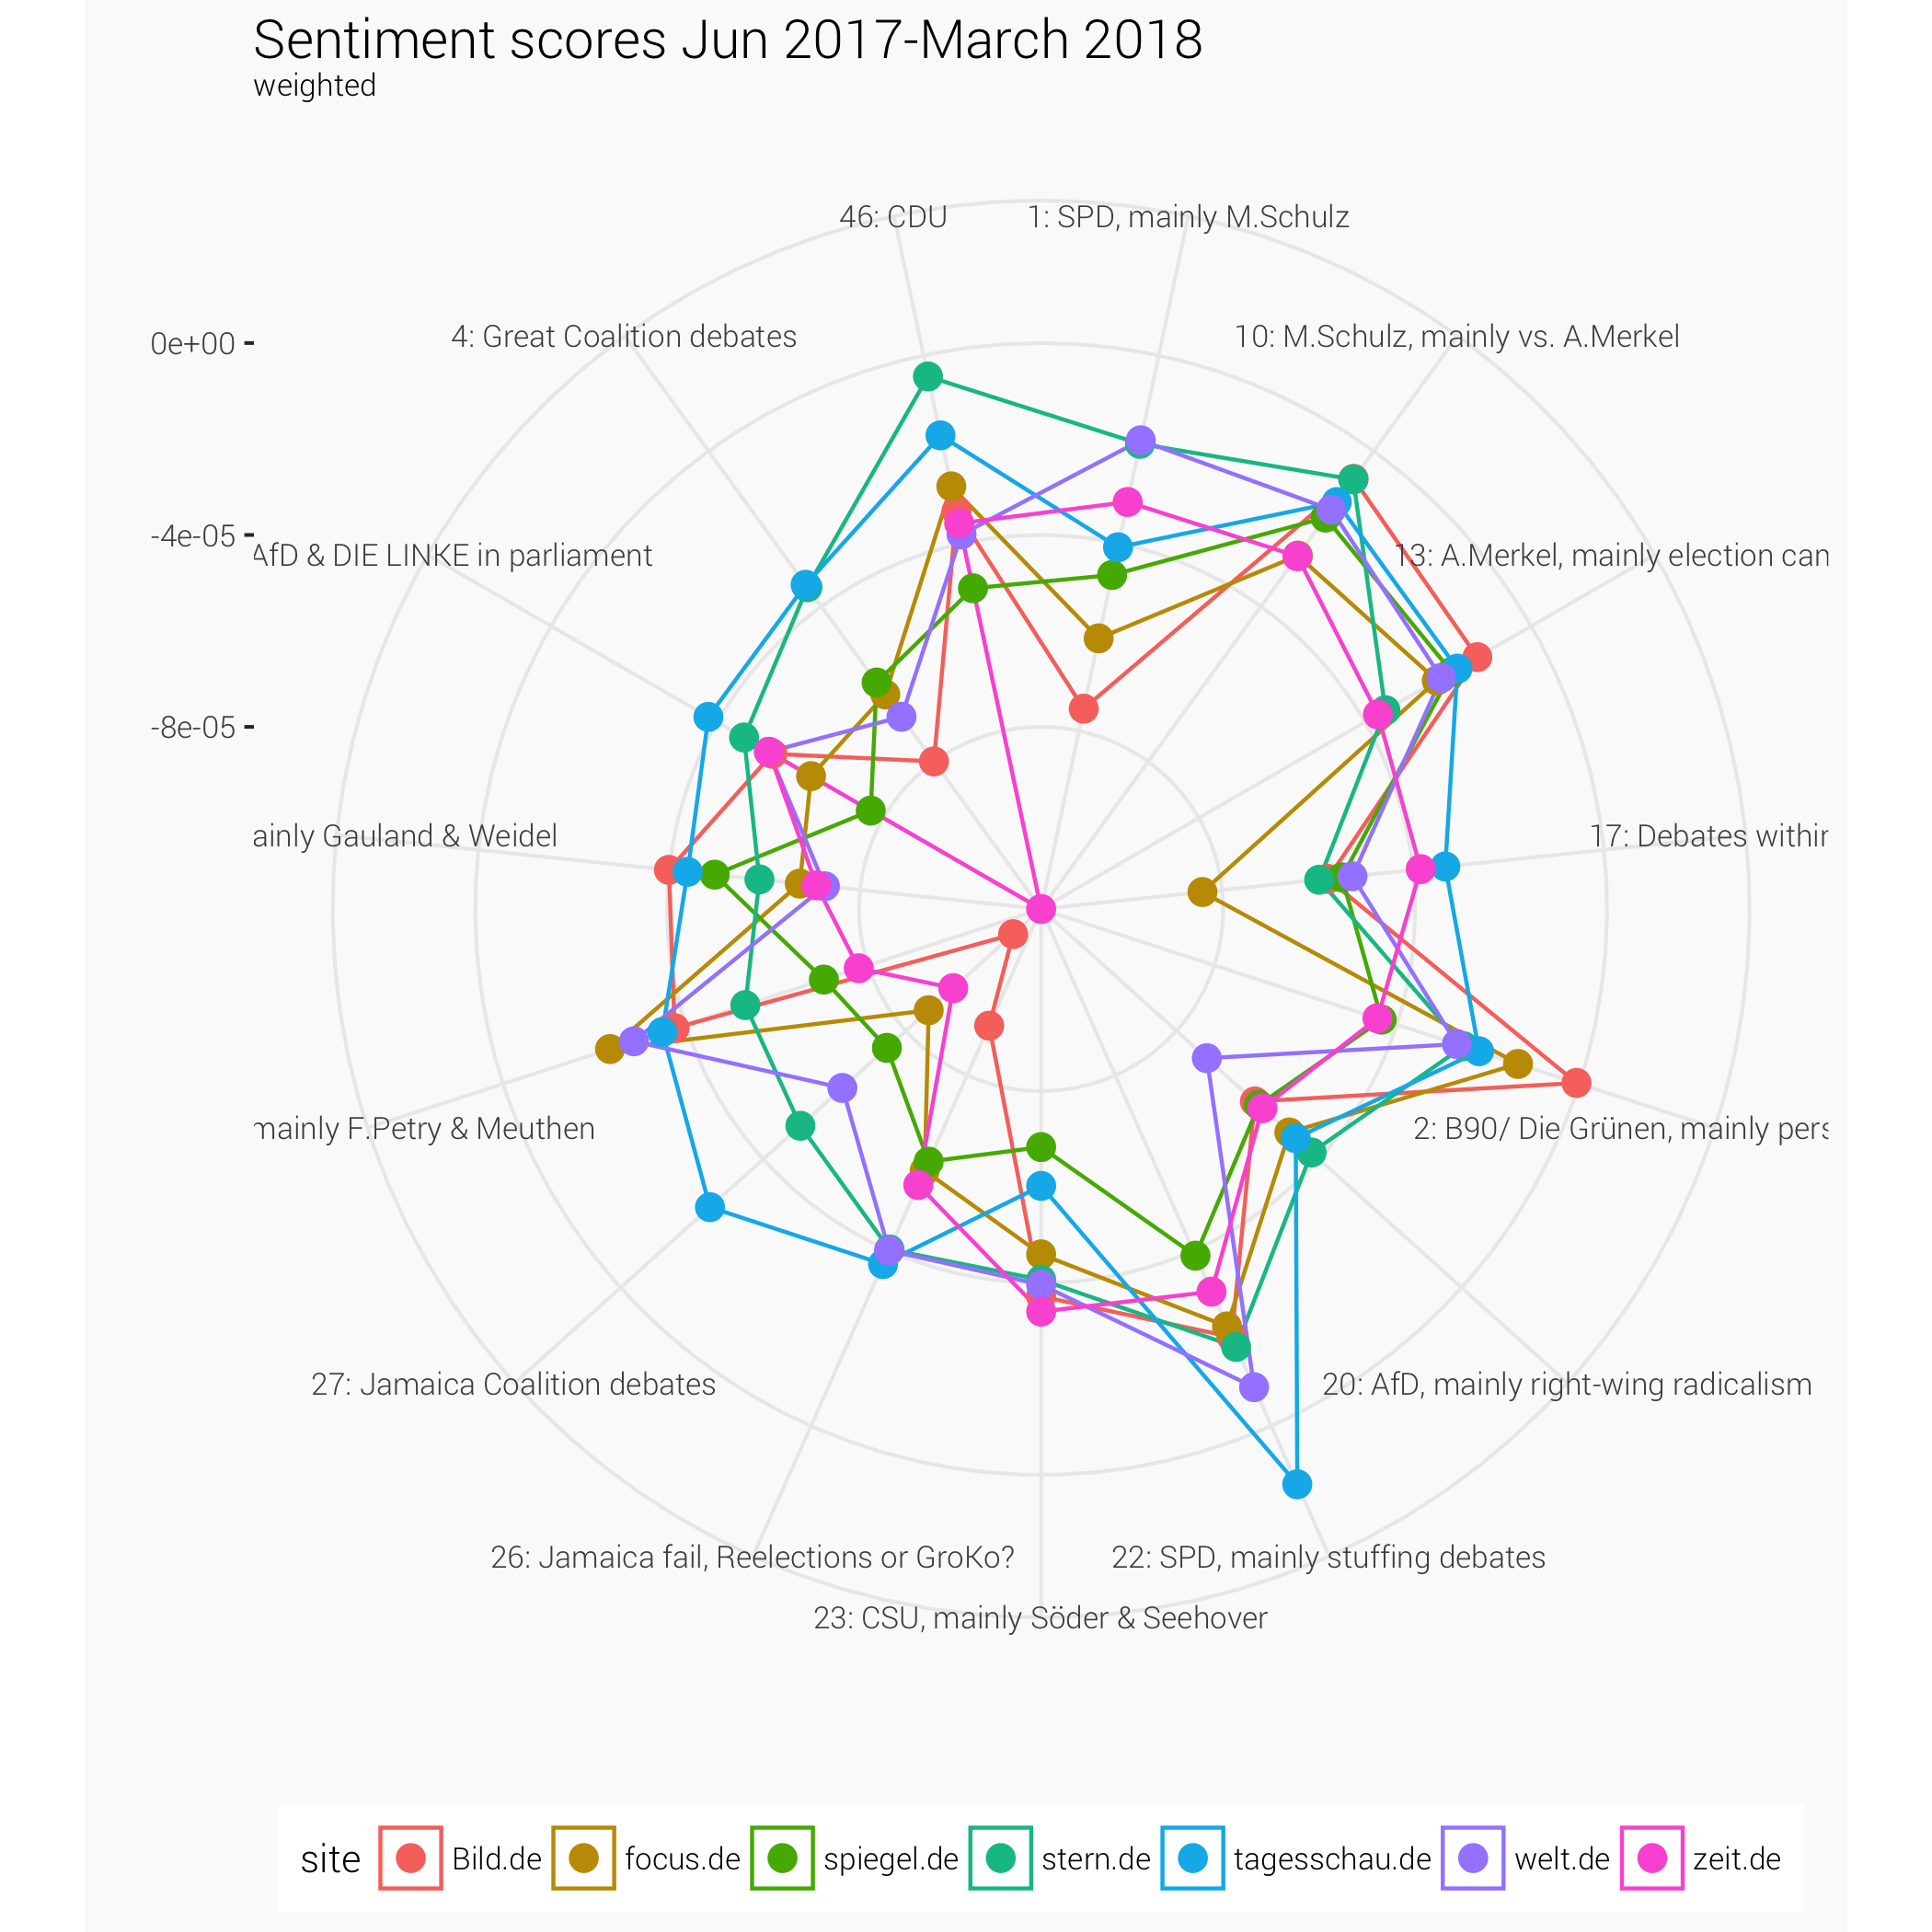
\includegraphics[width=\textwidth,keepaspectratio]{../figs/sentscore_radar.png}
			\label{fig_sentscore_radar}
		\end{subfigure}
		\end{center}
\end{figure}


% ----------------------
% Appendix
% ----------------------
\section*{Appendix}

\end{document}
